%%% ======= Beamer ======
\documentclass[usenames,dvipsnames,t]{beamer}
% \documentclass[usenames,dvipsnames, handout]{beamer}
\beamertemplatenavigationsymbolsempty % remove toolbar at the bottom of slides
\usepackage{appendixnumberbeamer} % for appendix
\usetheme{Madrid}
\usecolortheme{default}
\useinnertheme{circles}

\setbeamercolor{author in head/foot}{bg=blue!10, fg=blue}
\setbeamercolor{title in head/foot}{bg=blue!10, fg=blue}
\setbeamercolor{date in head/foot}{bg=blue!10, fg=blue}

\makeatletter
\setbeamertemplate{footline}{
  \leavevmode%
  \hbox{%
  \begin{beamercolorbox}[wd=.333333\paperwidth,ht=2.25ex,dp=1ex,center]{author in head/foot}%
    \usebeamerfont{author in head/foot}\insertshortauthor\expandafter\ifblank\expandafter{\beamer@shortinstitute}{}{~~(\insertshortinstitute)}
  \end{beamercolorbox}%
  \begin{beamercolorbox}[wd=.333333\paperwidth,ht=2.25ex,dp=1ex,center]{title in head/foot}%
    \usebeamerfont{title in head/foot}\insertshorttitle
  \end{beamercolorbox}%
  \begin{beamercolorbox}[wd=.333333\paperwidth,ht=2.25ex,dp=1ex,right]{date in head/foot}%
    \usebeamerfont{date in head/foot}\insertshortdate{}\hspace*{2em}
    \insertframenumber{}%
%     / \inserttotalframenumber
    \hspace*{2ex} 
  \end{beamercolorbox}}%
  \vskip0pt%
}
\makeatother

\colorlet{beamer@blendedblue}{blue!70} % change color theme

\usepackage[style=numeric-comp,sorting=none,backend=biber]{biblatex}%<- specify style
\addbibresource{references.bib}%<- specify bib file

\usepackage{svg}


% For appendix
% \newcommand{\backupbegin}{
%    \newcounter{framenumberappendix}
%    \setcounter{framenumberappendix}{\value{framenumber}}
% }
% \newcommand{\backupend}{
%    \addtocounter{framenumberappendix}{-\value{framenumber}}
%    \addtocounter{framenumber}{\value{framenumberappendix}} 
% }

\setbeamertemplate{bibliography item}{\insertbiblabel} % improved references



% Other preamble stuff:
\usepackage{preamble}

%%% Uncomment for another color palette
% \definecolor{Logo1}{rgb}{0.0, 0, 0.7}
% \definecolor{Logo2}{rgb}{2.55, 2.55, 2.55}

% \setbeamercolor*{palette primary}{bg=Logo1, fg=white}
% \setbeamercolor*{palette secondary}{bg=Logo2, fg=white}
% \setbeamercolor*{palette tertiary}{bg=white, fg=Logo1}
% \setbeamercolor*{palette quaternary}{bg=white,fg=white}
% \setbeamercolor{structure}{fg=Logo1} % itemize, enumerate, etc
% \setbeamercolor{section in toc}{fg=Logo1} % TOC sections

% For figures
\usepackage{import}
\usepackage{xifthen}
\usepackage{pdfpages}
\usepackage{transparent}
\usepackage{mdframed}
\usepackage{subcaption}

\setbeamertemplate{caption}[numbered]



% --- Inkscape figures:
\newcommand{\incfig}[2][0.75\textwidth]{%
    \def\svgwidth{\columnwidth}
    \resizebox{#1}{!}{\import{Inkscape figs/}{#2.pdf_tex}}
}

% --- Height of frame
\newlength{\myheight}
\setlength{\myheight}{7cm}


%------------------------------------------------------------
%This block of code defines the information to appear in the
%Title page
\title[Extreme matter/PE] %optional
{Robust parameter estimation on gravitational wave signals from binary neutron star inspirals within minutes}

\author[Thibeau Wouters]{\small{\textbf{Thibeau Wouters}, Peter T.H. Pang, Tim Dietrich, Chris Van Den Broeck} \\ \vspace{7mm} email: \href{mailto:t.r.i.wouters@uu.nl}{t.r.i.wouters@uu.nl} \\ \vspace{3mm} email: \href{https://arxiv.org/}{arXiv:????.??????}  }

\date{April 8, 2024}




%End of title page configuration block
%------------------------------------------------------------



%------------------------------------------------------------
%The next block of commands puts the table of contents at the 
%beginning of each section and highlights the current section:

% \AtBeginSection[]
% {
%   \begin{frame}[plain, noframenumbering]
%     \frametitle{Table of Contents}
%     \tableofcontents[currentsection]
%   \end{frame}
% }

% \AtBeginSubsection[]
% {
%   \begin{frame}[plain, noframenumbering]
%     \frametitle{Table of Contents}
%     \tableofcontents[currentsection]
%   \end{frame}
% }


%------------------------------------------------------------


\begin{document}

{

\usebackgroundtemplate{\transparent{0.15}{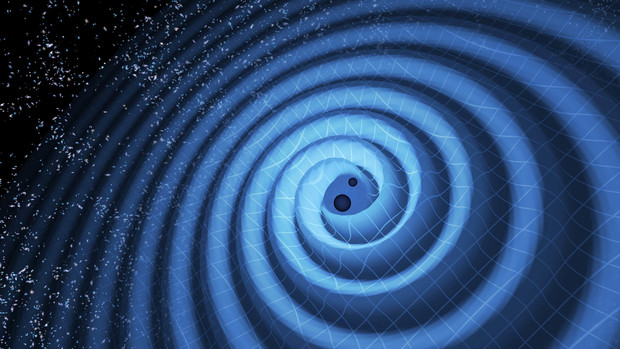
\includegraphics[width=\paperwidth,height=\paperheight]{Figures/GW-2.jpeg}}}

\begin{frame}[plain]
\titlepage

\begin{columns}
  \column{0.35\textwidth}
  \begin{figure}
    \centering
    \vspace{1.5mm}
    
\includegraphics[width=0.75\linewidth]{Figures/utrecht-university.png}
  \end{figure}
  \column{0.35\textwidth}
  \begin{figure}
    \centering
    
\includegraphics[width=0.75\linewidth]{Figures/Nikhef_logo-transparent.png}
  \end{figure}
\end{columns}


%%% as subfigures
% \begin{figure}
%   \centering
%   \begin{subfigure}[b]{0.475\textwidth}
%     \centering
%     
\includegraphics[width=0.6\textwidth]{Figures/utrecht-university.png}
%   \end{subfigure}
%   \caption*{}
%   \hfill
%   \begin{subfigure}[b]{0.475\textwidth}
%     \centering
%     
\includegraphics[width=0.6\textwidth]{Figures/Nikhef_logo-transparent.png}
%   \end{subfigure}
%   \caption*{}
%   % \caption*{}
% \end{figure}

\end{frame}
}

% %The next statement creates the title page.
% \frame[plain]{\titlepage



% }


%---------------------------------------------------------
%This block of code is for the table of contents after
%the title page
% \begin{frame}[plain, noframenumbering]
% \frametitle{Table of Contents}
% \tableofcontents
% \end{frame}
%---------------------------------------------------------


\section{Introduction}

\begin{frame}{Parameter estimation}

\def\x{3mm}
\def\y{2mm}

\begin{itemize}
    \item Parameter estimation (PE): get \red{posterior} of GW parameters $\theta$ % from data $d$
    \begin{equation*}
        \red{p(\theta | d)} = \frac{p(d | \theta) p(\theta)}{p(d)}
    \end{equation*}

    \vspace{\y}

    \item \textbf{Problem:} Markov Chain Monte Carlo (MCMC): computationally expensive for binary neutron stars (BNS)
    
\end{itemize}

% \vspace{\x}

\vspace{5mm}

\begin{figure}
  \centering
  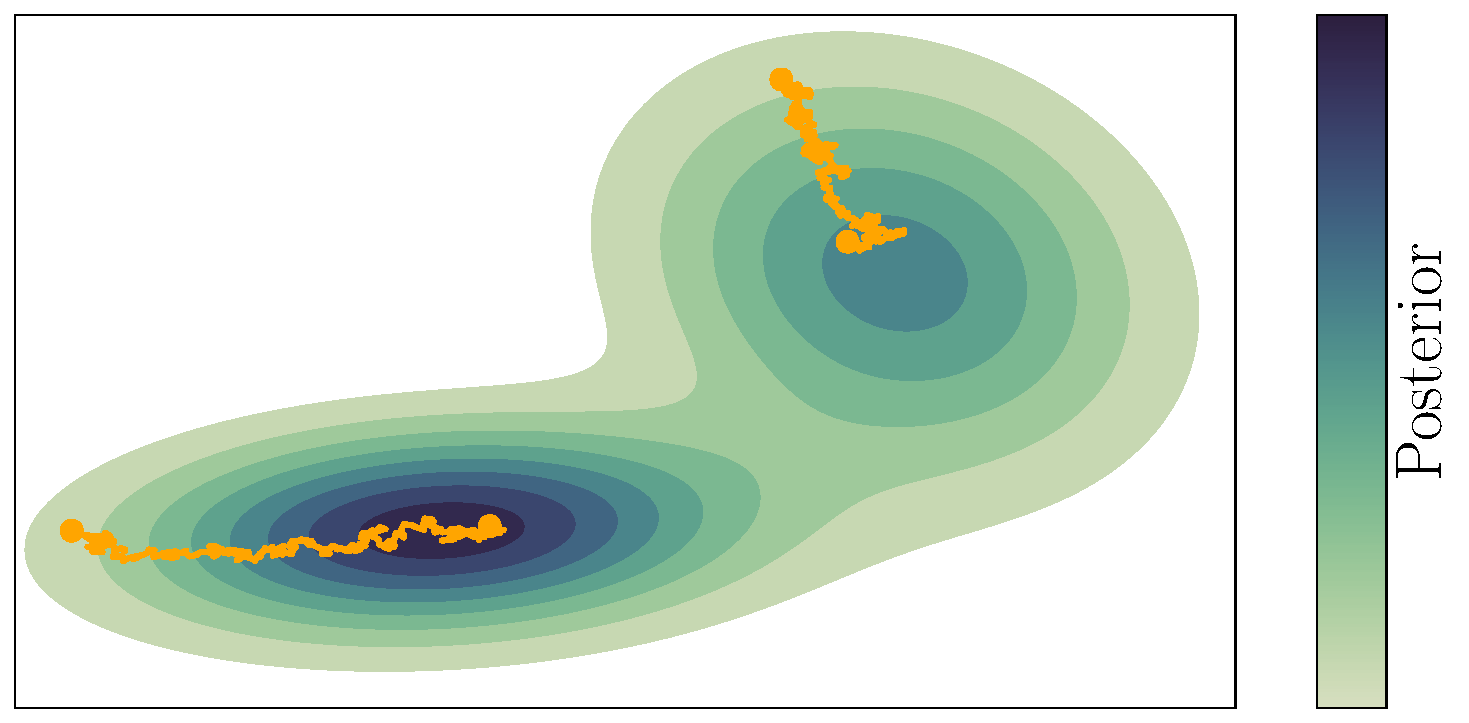
\includegraphics[width=0.7\textwidth]{Figures/mixture_of_gaussians_projection_no_title_colorbar.pdf}
  \caption*{}
\end{figure}

\end{frame}


\begin{frame}{Methods}

\def\xx{1mm}
\def\x{3mm}
\def\y{2mm}
\def\z{-0mm}

We extend \textsc{Jim}~\cite{wong2023fast} to analyze BNS signals:

\vspace{\xx}

\begin{itemize}
  \item \textsc{jax}: automatic differentiation, GPU acceleration~\cite{frostig2018compiling}
  
  \vspace{\x}
  
  \item Waveforms: \texttt{TaylorF2} and \texttt{IMRPhenomD\_NRTidalv2} in \textsc{ripple}~\cite{edwards2023ripple}
  
  \vspace{\x}

  \item Relative binning: speed up likelihood evaluation~\cite{Krishna:2023bug, Zackay:2018qdy}

  \vspace{\x}
  
  \item MCMC sampler: \textsc{flowMC}~\cite{wong2022flowmc}
  \vspace{\y}
  \begin{itemize}
    \item Gradient-based sampler: ``local sampler"
  
    \vspace{\y}

    \item Normalizing flows (NF):  ``global sampler"
  \end{itemize}
\end{itemize}

\vspace{\z}


\begin{figure}
  \centering
  \incfig[\textwidth]{flowMCOverview2}
  \caption*{}
\end{figure}
\end{frame}


\begin{frame}{Validation -- p-p plot}
  
  \def\x{1mm}
  \def\y{3mm}

  We demonstrate the robustness of \textsc{Jim}:

  \begin{itemize}
    \item 100 GW events with HLV at design sensitivity and $T = 128$ s,
    
    \vspace{\x}

    \item \texttt{NRTv2}: reference waveform relative binning without taper,
    
    \vspace{\x}
    
    \item Priors: Table~\ref{tab:parameter_priors}.
  \end{itemize}


  \begin{columns}
    \column{0.49\textwidth}
    \begin{figure}
      \centering
      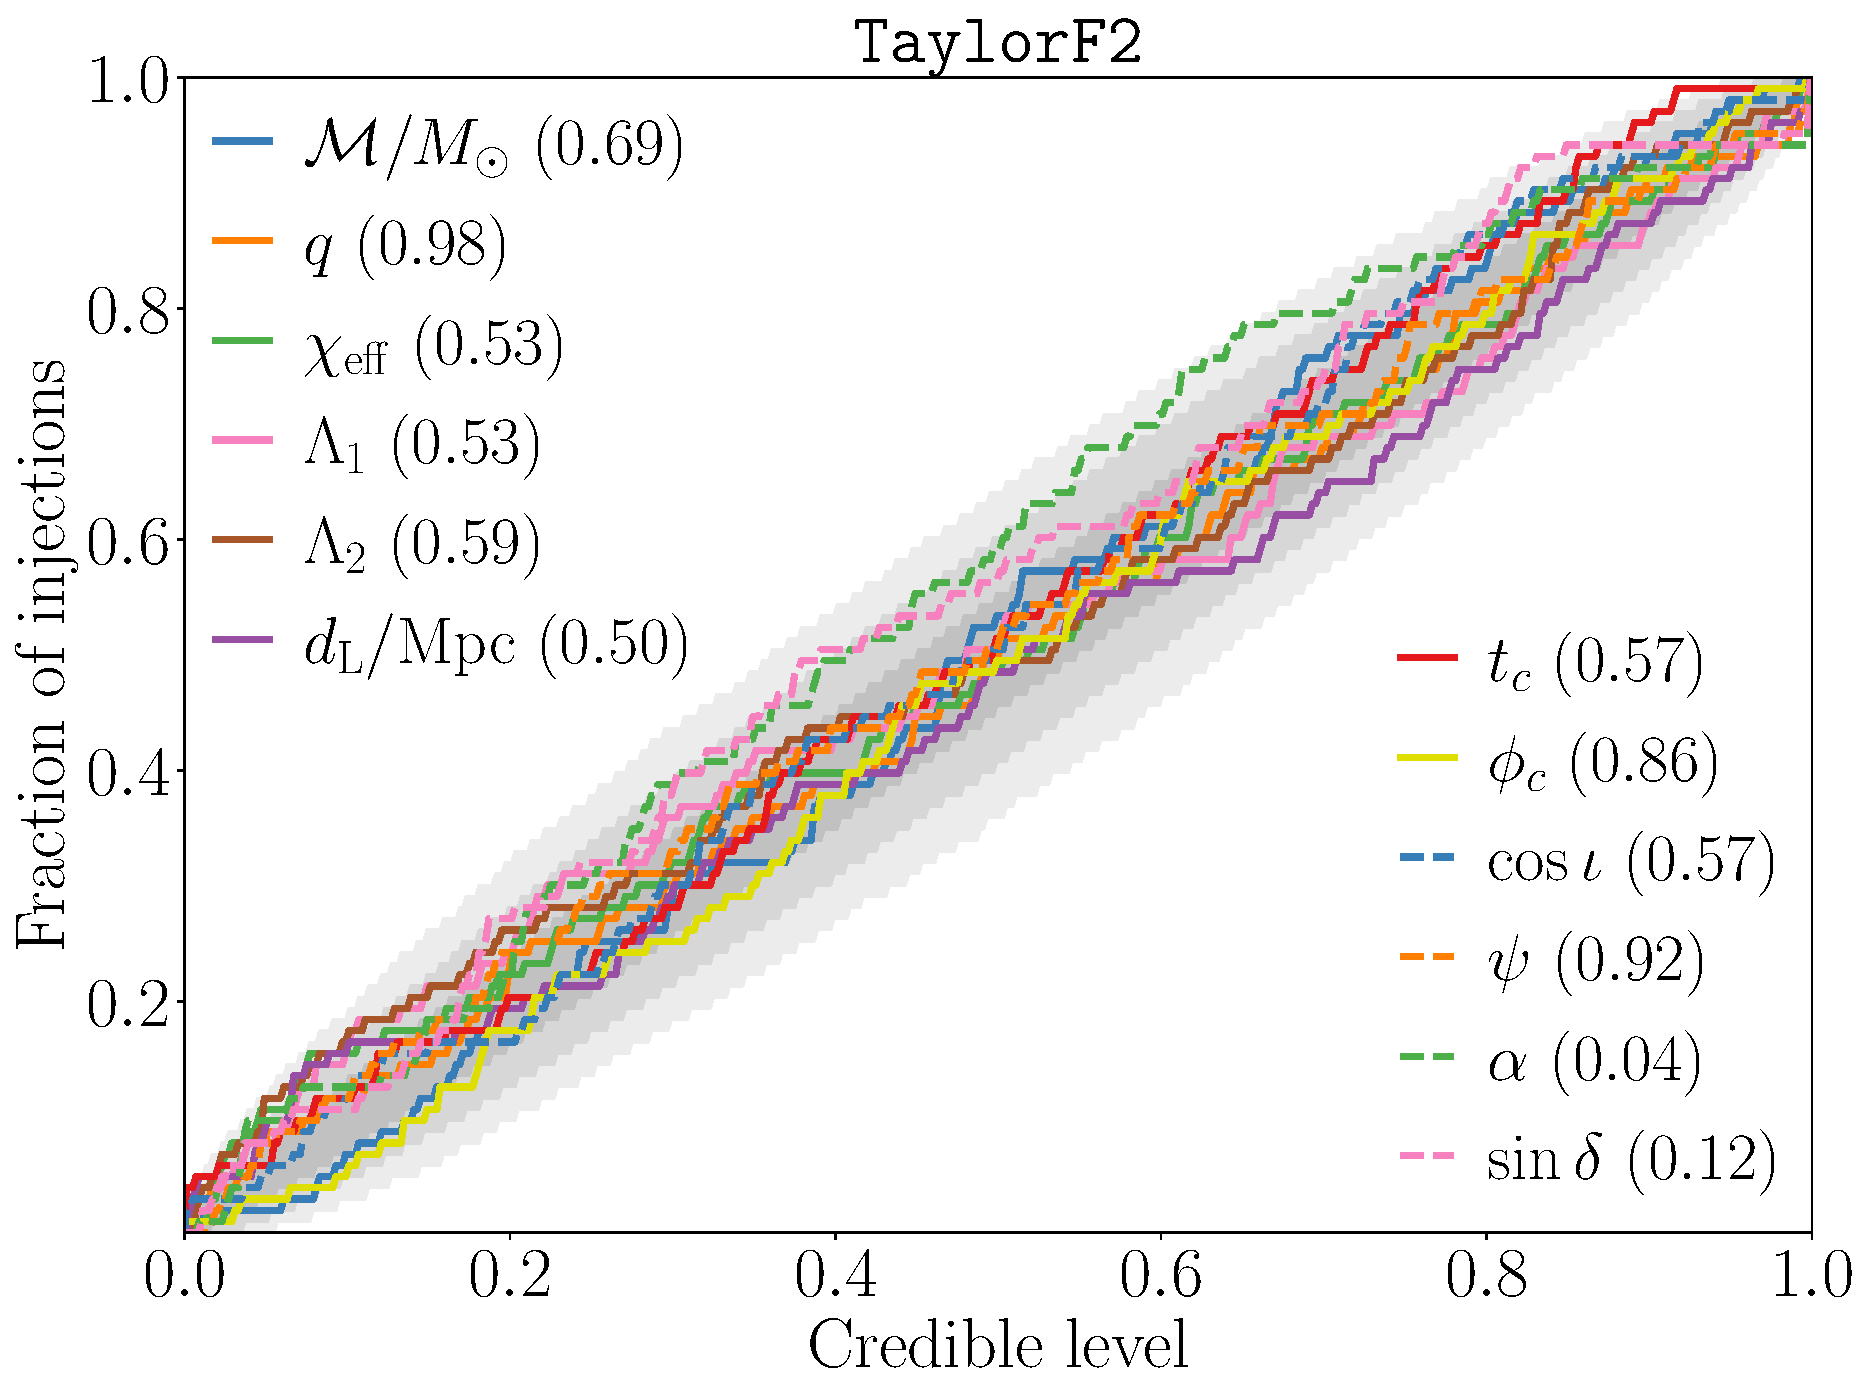
\includegraphics[width=\linewidth]{Figures/pp_plot_TF2.pdf}
    \end{figure}
    \column{0.49\textwidth}
    \begin{figure}
      \centering
      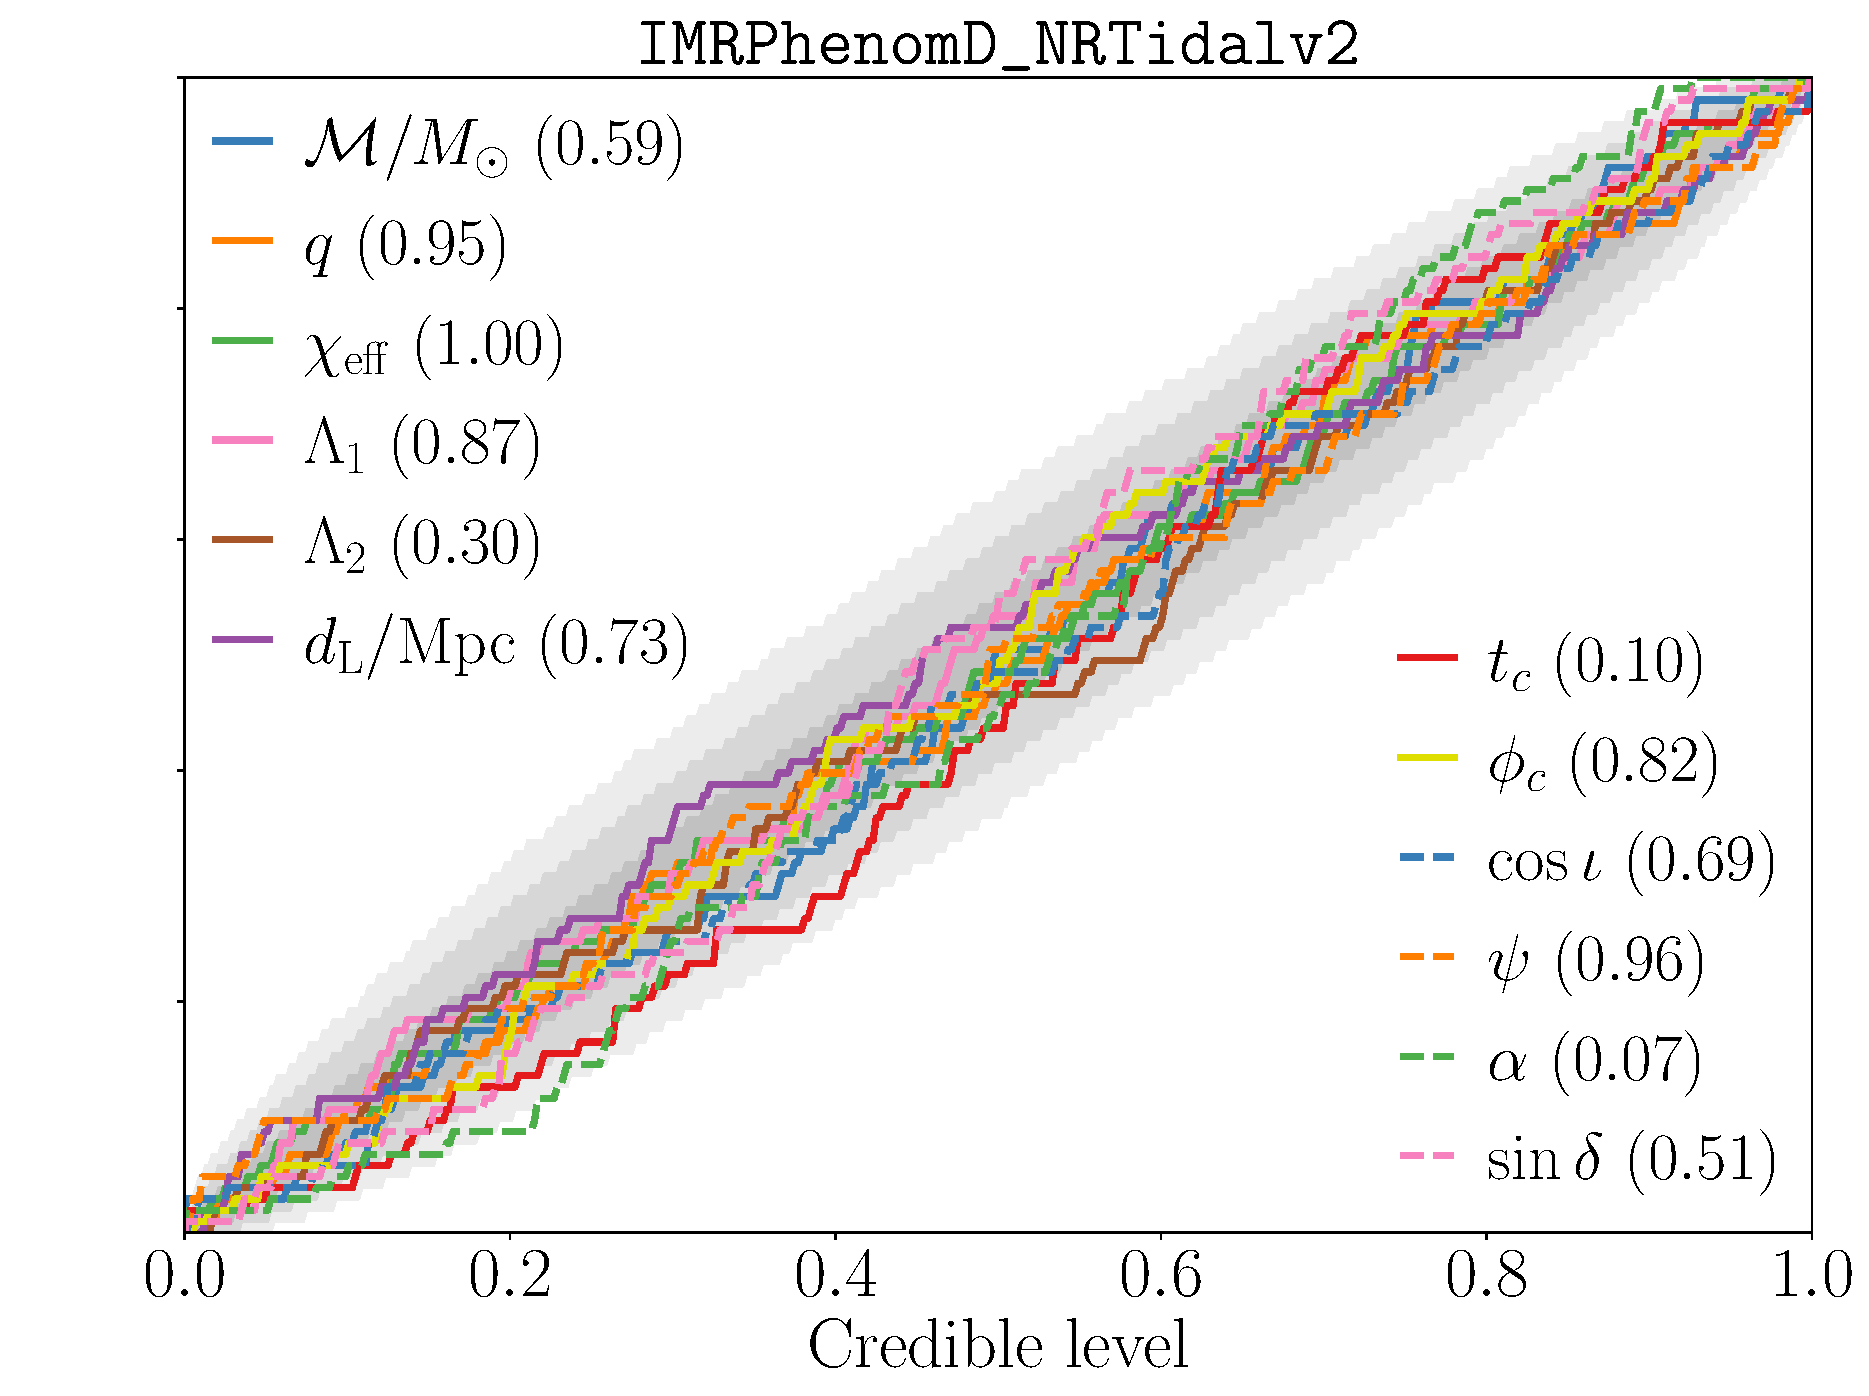
\includegraphics[width=\linewidth]{Figures/pp_plot_NRTv2.pdf}
    \end{figure}
  \end{columns}
  
  % \begin{figure}
  %   \begin{subfigure}[t]{0.475\textwidth}
  %     \centering
  %     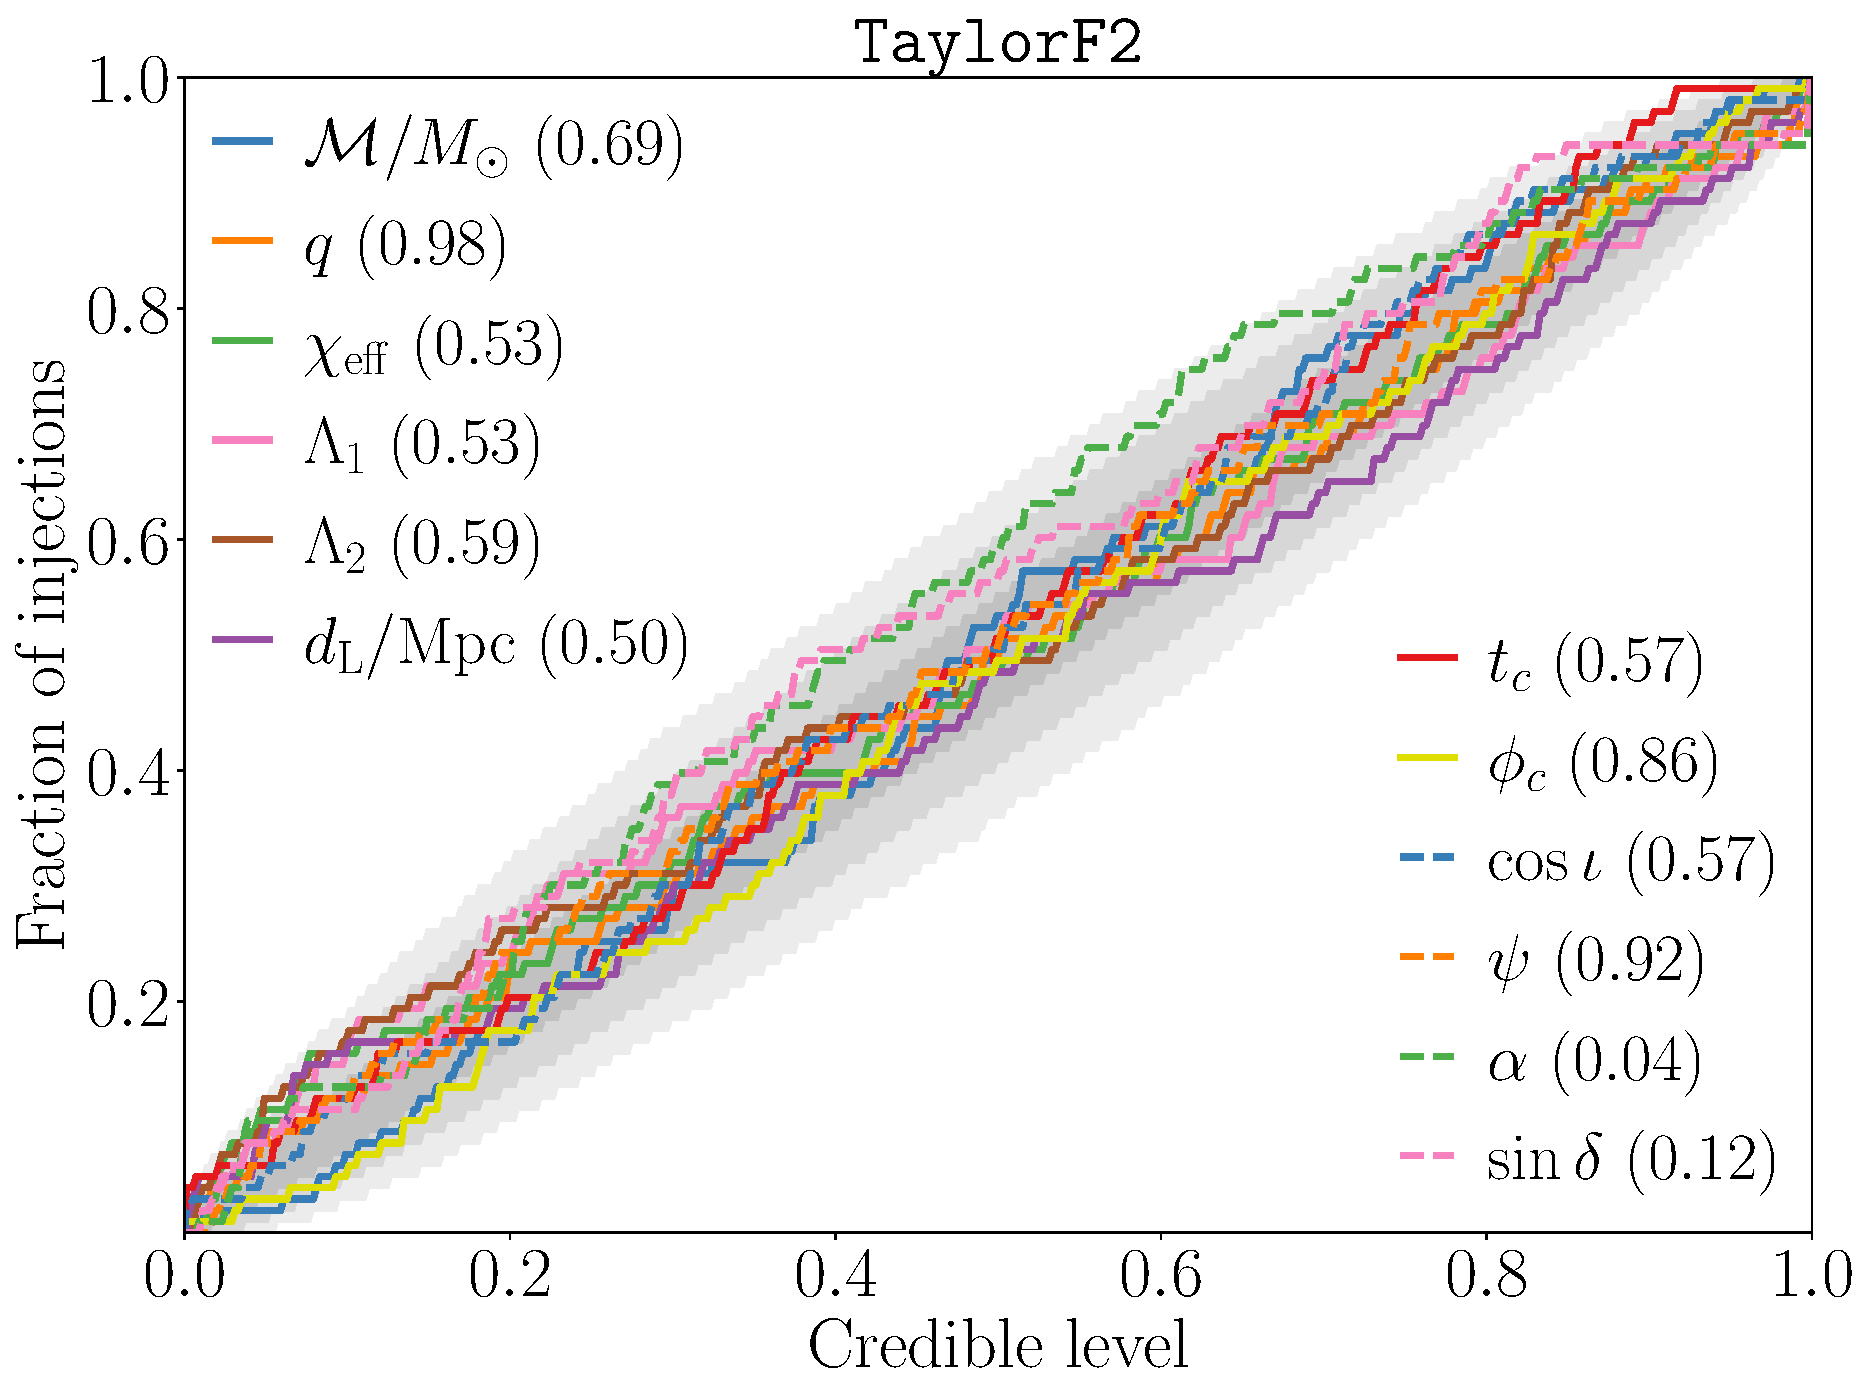
\includegraphics[width=\textwidth]{Figures/pp_plot_TF2.pdf}
  % \end{subfigure}
  % \hfill
  % \begin{subfigure}[t]{0.475\textwidth}
  %     \centering
  %     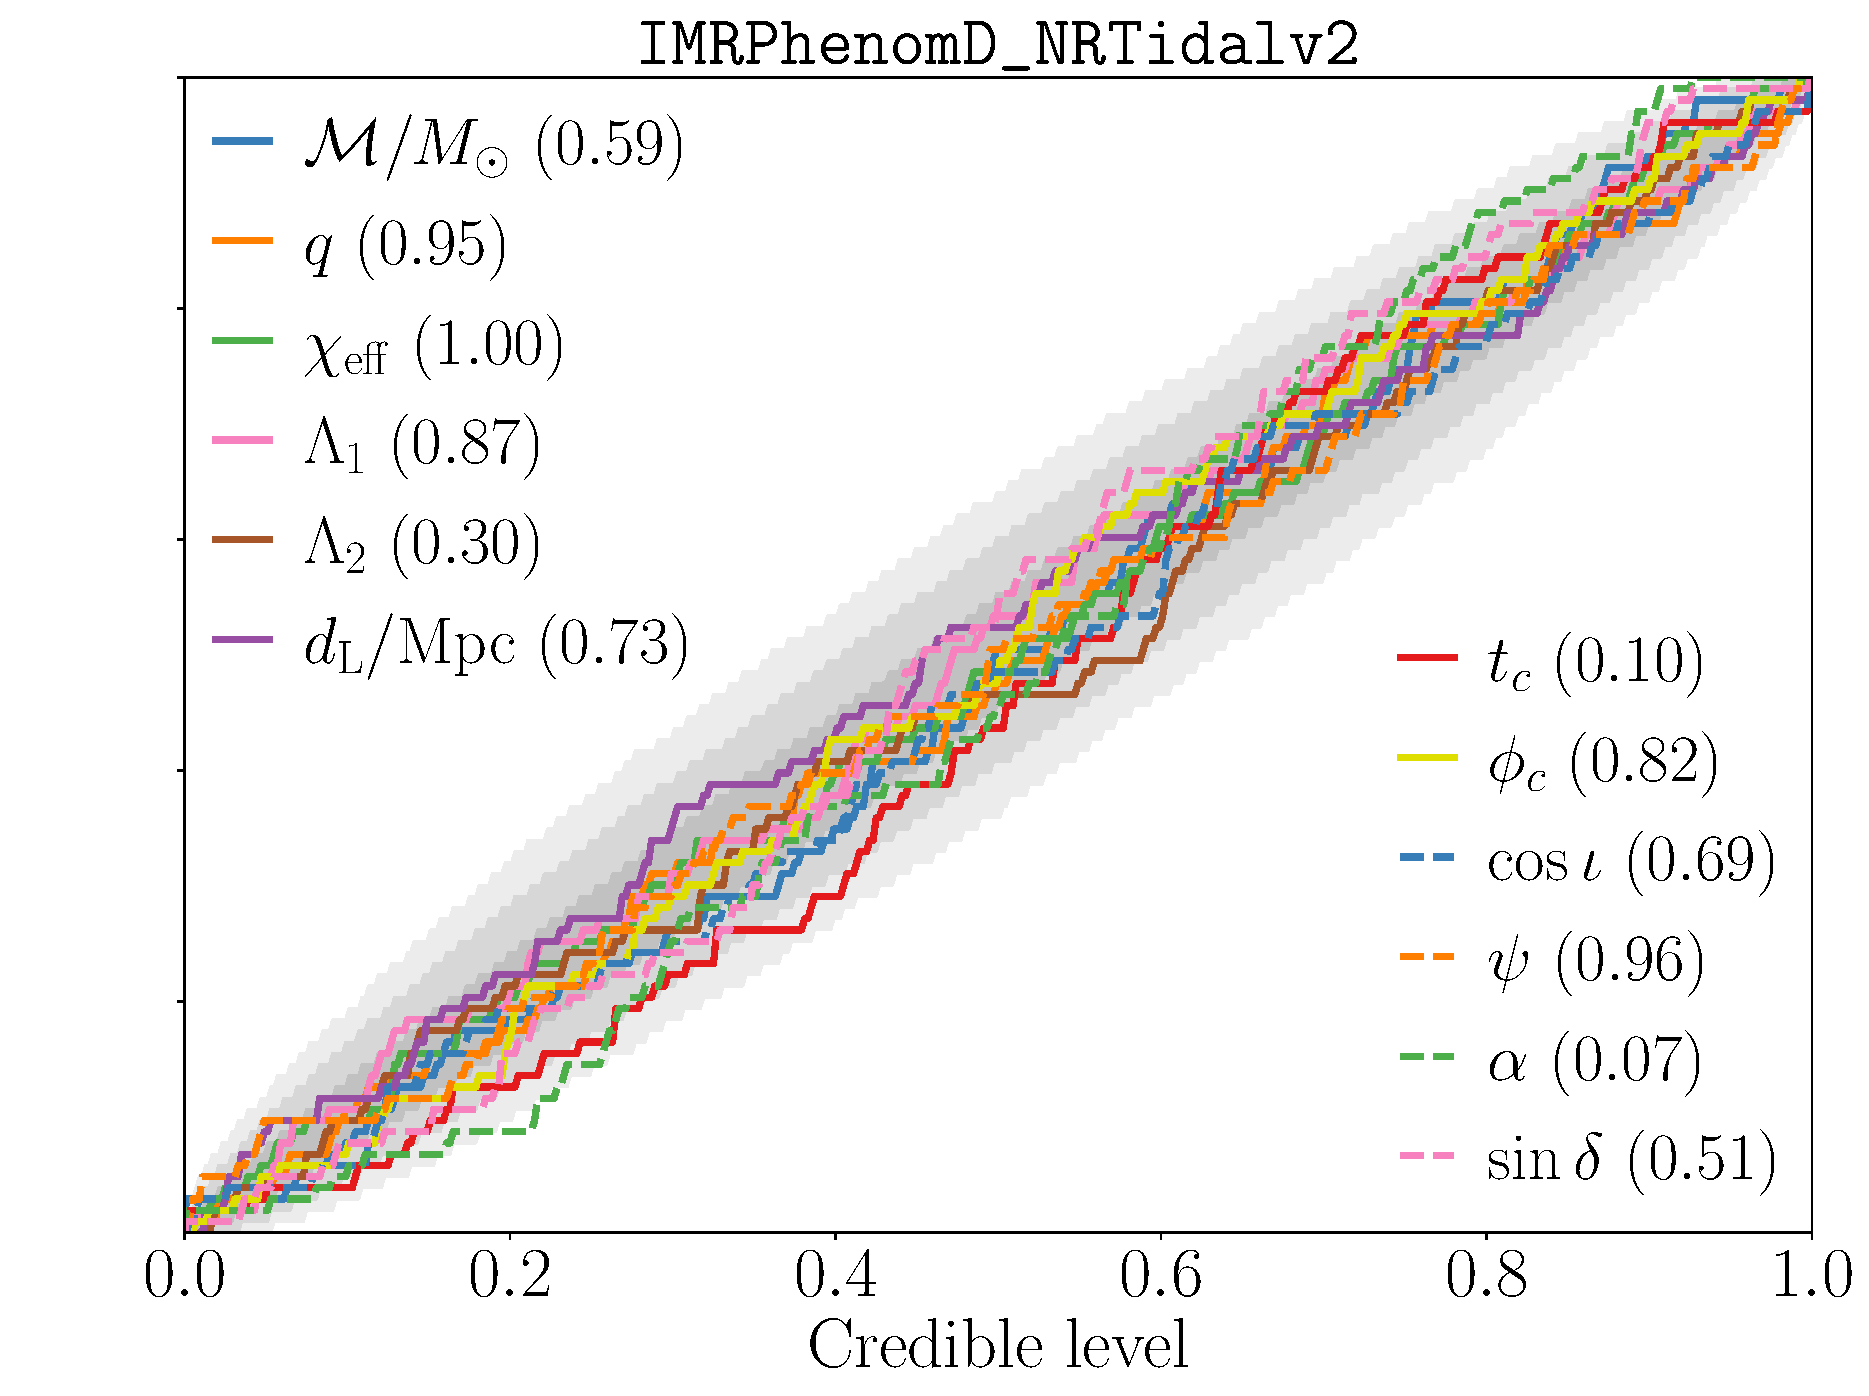
\includegraphics[width=\textwidth]{Figures/pp_plot_NRTv2.pdf}
  % \end{subfigure}
  % %  \caption{\ac{p-p} plot for the injections done with \texttt{TaylorF2} (left) and \texttt{IMRPhenomD\_NRTidalv2} (right), each created from 100 injections. For both of the waveform models, the \ac{p-p} plots are agreeing well with the diagonal, demonstrating the robustness of the \textsc{Jim} pipeline on analyzing \ac{BNS} signals.}
  % %  \label{fig:pp plots}
  % \caption*{}
  % \end{figure}
  
\end{frame}




\begin{frame}{Results -- GW170817 \& GW190425}
  % \begin{minipage}[c]{0.2\textwidth}
  % \caption{GW170817 with \texttt{TaylorF2}}\label{fig: GW170817 TaylorF2 first plot}
  % \end{minipage}\hfill
  % \begin{minipage}[c]{0.8\textwidth}
    % \end{minipage}

    \def\x{3mm}

    \begin{columns}
      \column{0.325\textwidth}
      \begin{itemize}
        \item Compare with \textsc{pBilby}

        \vspace{\x}
        
        \item Cornerplots: Figure~\ref{fig: GW170817 TaylorF2},~\ref{fig: GW170817 NRTidalv2},~\ref{fig: GW190425 TaylorF2},~\ref{fig: GW190425 NRTidalv2}

        \vspace{\x}
  
        \item Jensen-Shannon divergences: Table~\ref{tab: JS divergences events}
        
        \vspace{\x}
        \item GW170817, \texttt{TaylorF2}:
      \end{itemize}


      \column{0.675\textwidth}
    \vspace{-15.5mm}
    \begin{figure}
    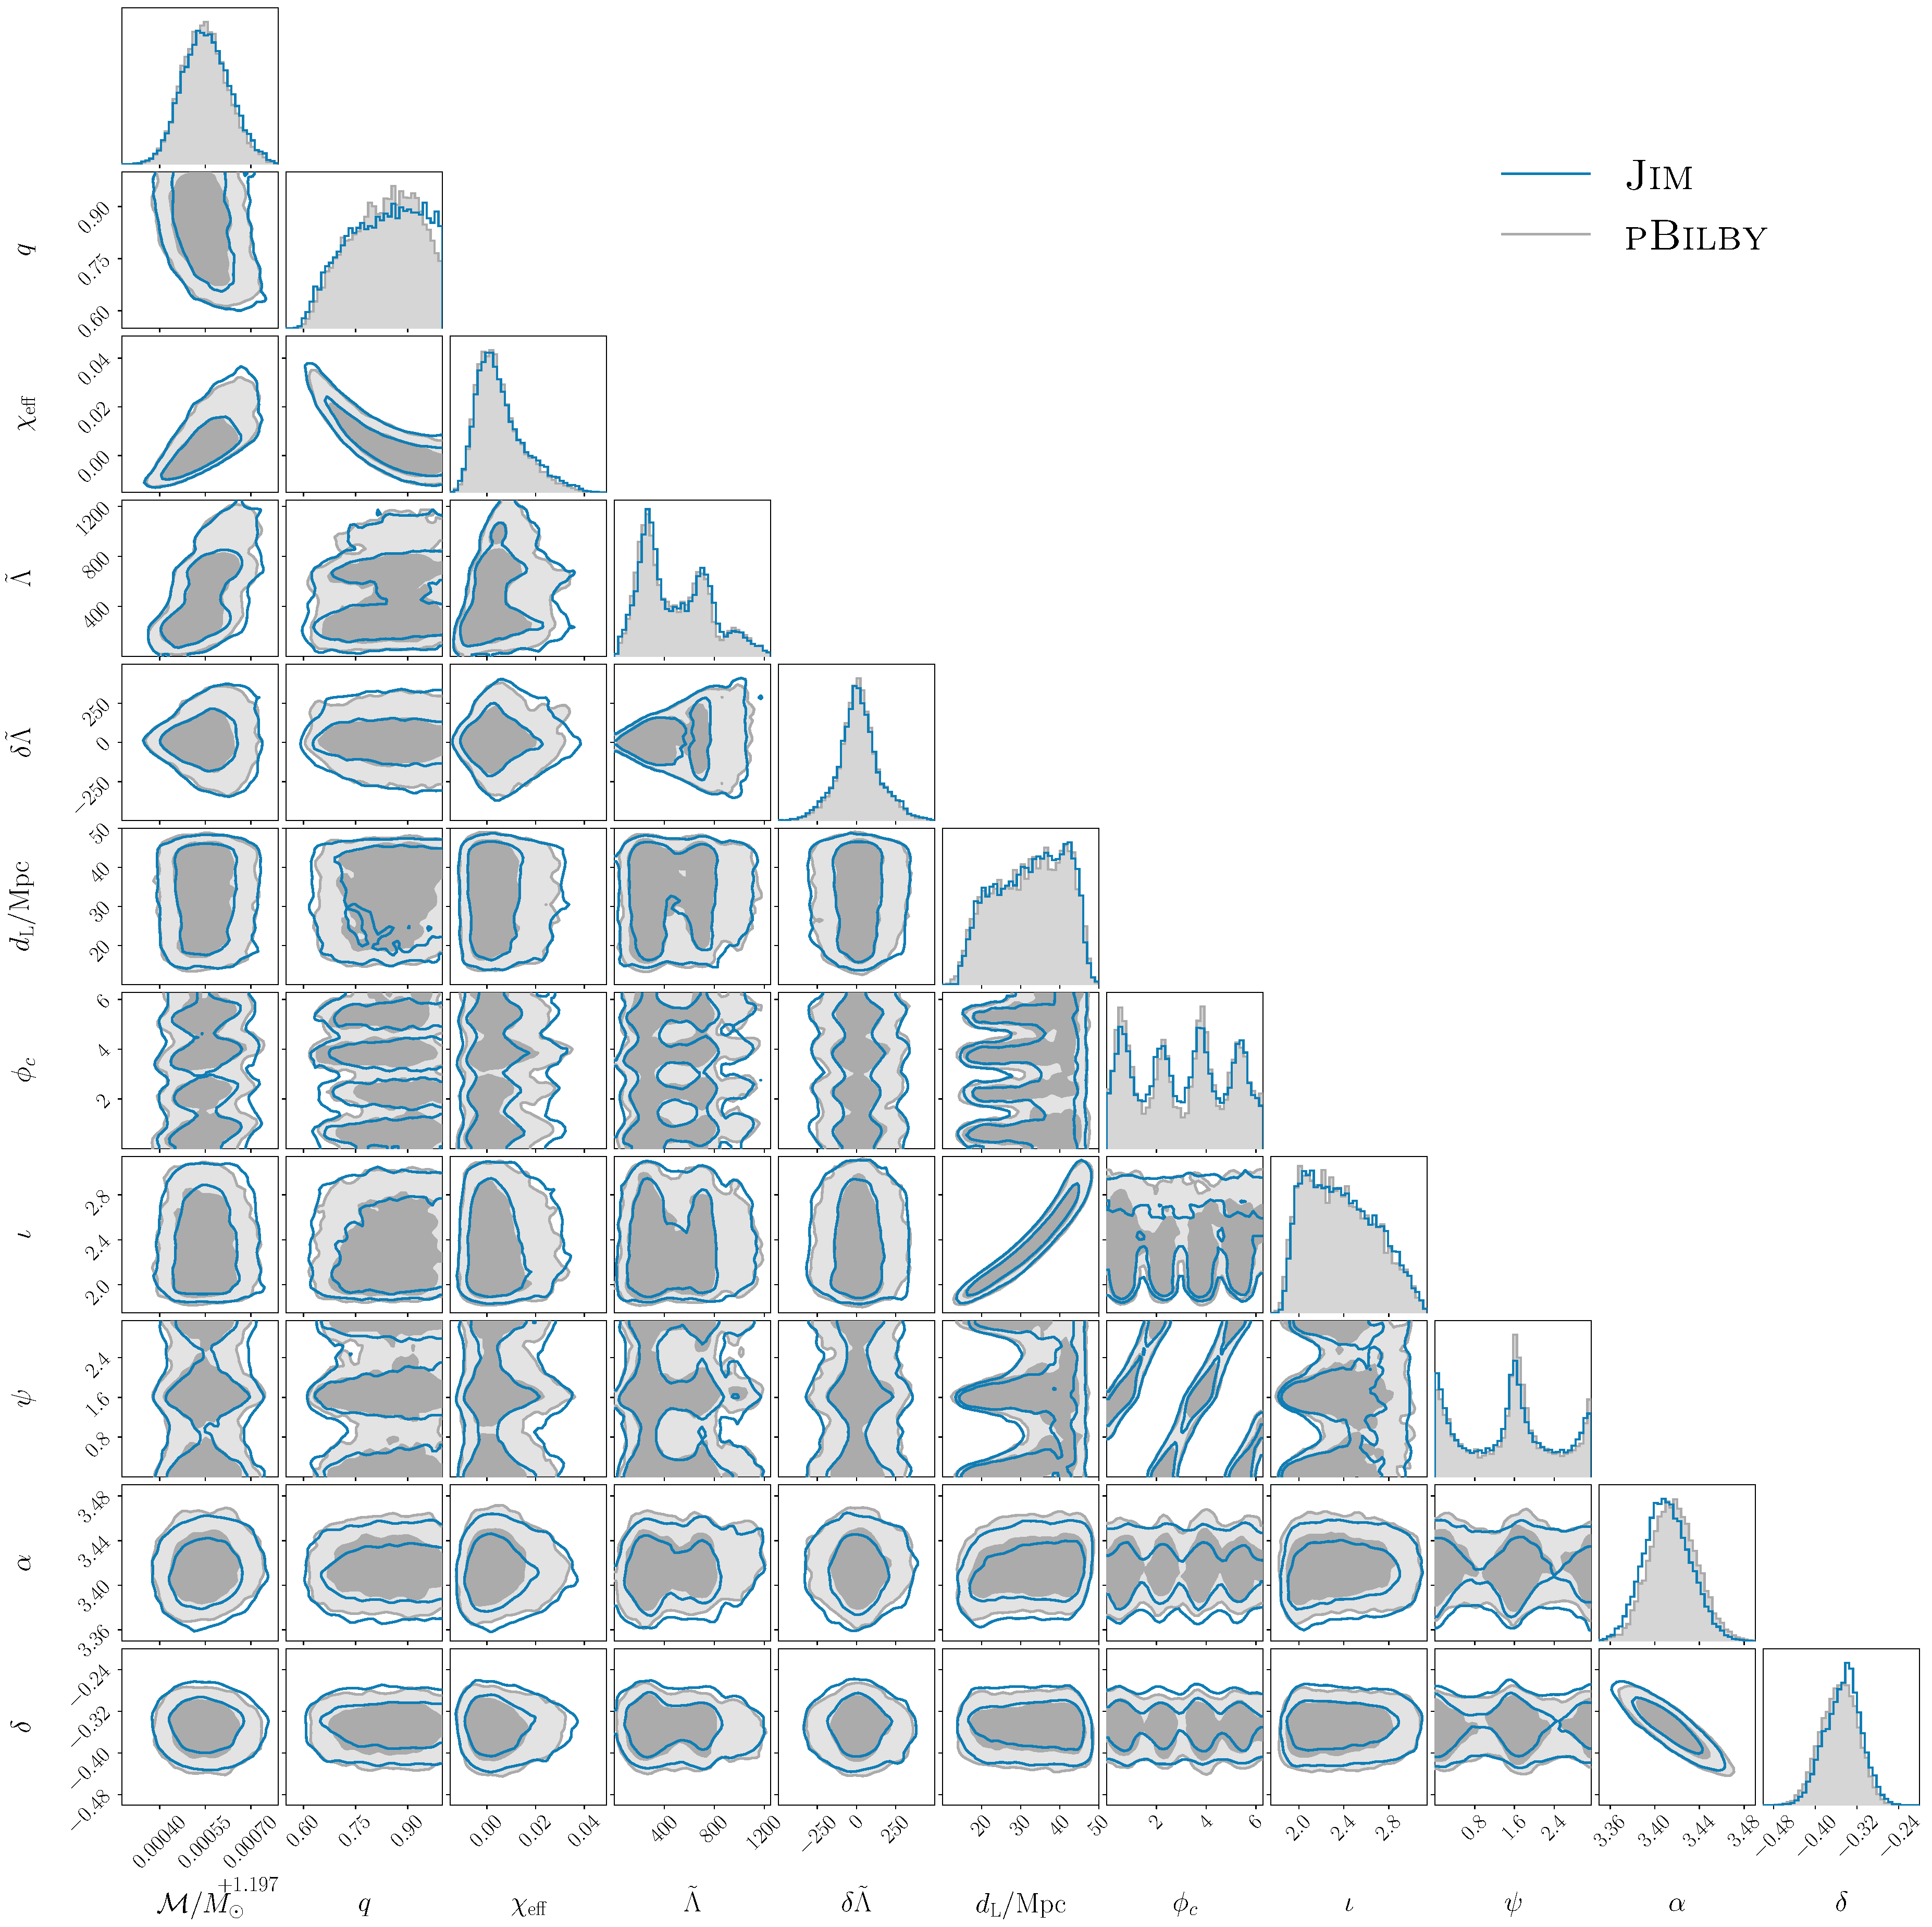
\includegraphics[scale = 0.132]{Figures/GW170817_TaylorF2.pdf}
    \caption*{}
    \end{figure}
    \end{columns}
    
  
\end{frame}


\begin{frame}{Results -- Runtime}

  \def\x{1mm}
  \def\y{3mm}

  \begin{itemize}
    \item Real events: includes (i) runtime to compute reference parameters for relative binning, (ii) training NF, (iii) sampling
    
    \vspace{\x}

    \item Injections: median runtime
    
    \vspace{\x}
    
    \item  1 GPU \footnotesize (A100) \normalsize -- vs -- 480 cores \footnotesize{(Intel Skylake Xeon Platinum $8174$)} \normalsize
    
  \end{itemize}
  
  \vspace{\y}

  \begin{table}
    \centering
    \renewcommand{\arraystretch}{1.4}
    \begin{tabular*}{0.975\linewidth}{@{\extracolsep{\fill}} l l c c c}
 Event & WF & \textsc{Jim} \footnotesize{($1$ GPU)} & \textsc{pBilby} \footnotesize{($480$ cores)} \\
  \hline\hline
 \multirow{2}{*}{GW170817} & \texttt{TF2} & $(9.70 + 17.00)$ min & $\phantom{0}9.64$ h \\
 & \texttt{NRTv2} & $(5.69 + 28.02)$ min & $10.99$ h \\ \hline
\multirow{2}{*}{GW190425}  & \texttt{TF2} & $(5.13 + 16.49)$ min & $\phantom{0}4.08$ h \\ 
 & \texttt{NRTv2} & $(6.15 + 15.37)$ min & $\phantom{0}4.69$ h \\ \hline
\multirow{2}{*}{Injection} & \texttt{TF2} & $\phantom{(0.000 + } 24.76\phantom{)}$ min & --  \\
& \texttt{NRTv2} & $\phantom{(0.000 + } 18.02\phantom{)}$ min & --  \\
\hline\hline
    \end{tabular*}
    % \caption{Total wall time spent on conducting \ac{PE} on the events mentioned in this work, with the \texttt{TaylorF2} (\texttt{TF2}) and \texttt{IMRPhenomD\_NRTidalv2} (\texttt{NRTv2}) waveform models. \textsc{Jim} is benchmarked on an NVIDIA A100 GPU. \textsc{pBilby} is benchmarked on $10$ Intel Skylake Xeon Platinum 8174, in total $480$ cores are used per run. For the real events analyzed with \textsc{Jim}, we quote the time spent on \textsc{evosax} and \textsc{flowMC} separately. For the injections, we quote the median value.}
    % \label{tab: runtimes table}
\end{table}
\end{frame}

\begin{frame}{Discussion -- environmental impact}
  
  \def\x{3mm}
  \def\y{3mm}

  \textsc{Jim} is $100 \times$ more environmentally friendly than \textsc{pBilby}

  \vspace{\x}

  \begin{itemize}
    \item Energy consumption for all $204$ runs
    
    \vspace{\x}

    \item Power of GPU: $400$W, power of CPU: $240$W
    
    \vspace{\x}

    \item Average NL household: ${2 \ 810}$ kWh/year
  \end{itemize}
  
  \vspace{\y}

  \begin{table}
    \centering
    \renewcommand{\arraystretch}{1.2}
    \begin{tabular*}{0.9\linewidth}{@{\extracolsep{\fill}} l r r r }
      & kWh & $\rm{CO}_2$ [$10^3$ kg] & Trees${}^\dagger$ \\
      \hline\hline
      \textsc{Jim} & $\phantom{00}33.78$ & $\phantom{0}0.01$ & $\phantom{000}0.55$ \\
      \textsc{pBilby} & $3598.53$ & $1.18$ & $59.02$ \\
     \hline\hline
    \end{tabular*}
    % \caption{Estimate of the environmental impact of performing all runs in this work with the \textsc{Jim} and \textsc{pBilby} pipelines. }
    % \label{tab: environmental impact}
\end{table}

${}^\dagger$Number of trees needed to capture the emitted $\rm{CO}_2$ in a year.

\end{frame}

\begin{frame}{Conclusion}

  \def\x{3mm}
  \def\y{2mm}

  \textsc{Jim}: a fast and environmentally friendly PE pipeline for GW signals
  
  \vspace{\y}

  \begin{itemize}
    \item Enhance MCMC with
    \begin{itemize}
      \vspace{\y}
      \item \textsc{jax},
      \vspace{\y}
      \item relative binning,
      \vspace{\y}
      \item gradient-based samplers, and
      \vspace{\y}
      \item normalizing flows
    \end{itemize}
    
    
    \vspace{\x}

    \item Analyze BNS in $15$ -- $30$ minutes of sampling time
    
    \vspace{\x}

    \item $100 \times$ more environmentally friendly than \textsc{pBilby}

    \vspace{\x}

    \item Science cases:
    \begin{itemize}
      \vspace{\y}
      \item low-latency alerts,

      \vspace{\y}

      \item large-scale population studies, and future generation GW detectors
    \end{itemize}
    
  \end{itemize}
\end{frame}

\begin{frame}{References}

\printbibliography
    
\end{frame}

% ======== APPENDIX  ==========

% \appendix

\begin{frame}{}
\vfill
\centering
\textbf{APPENDIX}
\vfill
\end{frame}

\begin{frame}{Normalizing flow}

  \def\x{4mm}

  Normalizing flows details: 

  \vspace{\x}

  \begin{itemize}
    \item Rational-quadratic neural spline flows
    
    \vspace{\x}
    
    \item 10 layers, 8 bins
    
    \vspace{\x}
    
    \item 128 neurons in hidden layers
    
    \vspace{\x}
    
    \item Adam optimizer, learning rate decayed (polynomial schedule)
    
    \vspace{\x}
    
    \item Deep learning library: \textsc{Equinox}~\cite{kidger2021equinox}
  \end{itemize}
  
\end{frame}

\begin{frame}{Validation -- Mismatch waveforms}

  Cross-check against \textsc{LALsuite}: mismatch histogram based on $10 \ 000$ waveforms, from uniform samples with following ranges:

  \footnotesize
  \begin{table}
    \centering
    \renewcommand{\arraystretch}{1.0}
    \begin{tabular}{l l} 
        \hline\hline
        Parameter & Range \\
        \hline
        Component masses & $[0.5M_{\odot}, 3M_{\odot}]$\\
        Component aligned spins & $[-0.05, 0.05]$\\
        Dimensionless tidal deformabilities &  $[0, 5000]$\\
        Inclination angle & $[0, \pi]$\\
        \hline\hline
    \end{tabular}
    \caption*{}
\end{table}
\normalsize

\vspace{-11.75mm}

  \begin{figure}
    \centering
    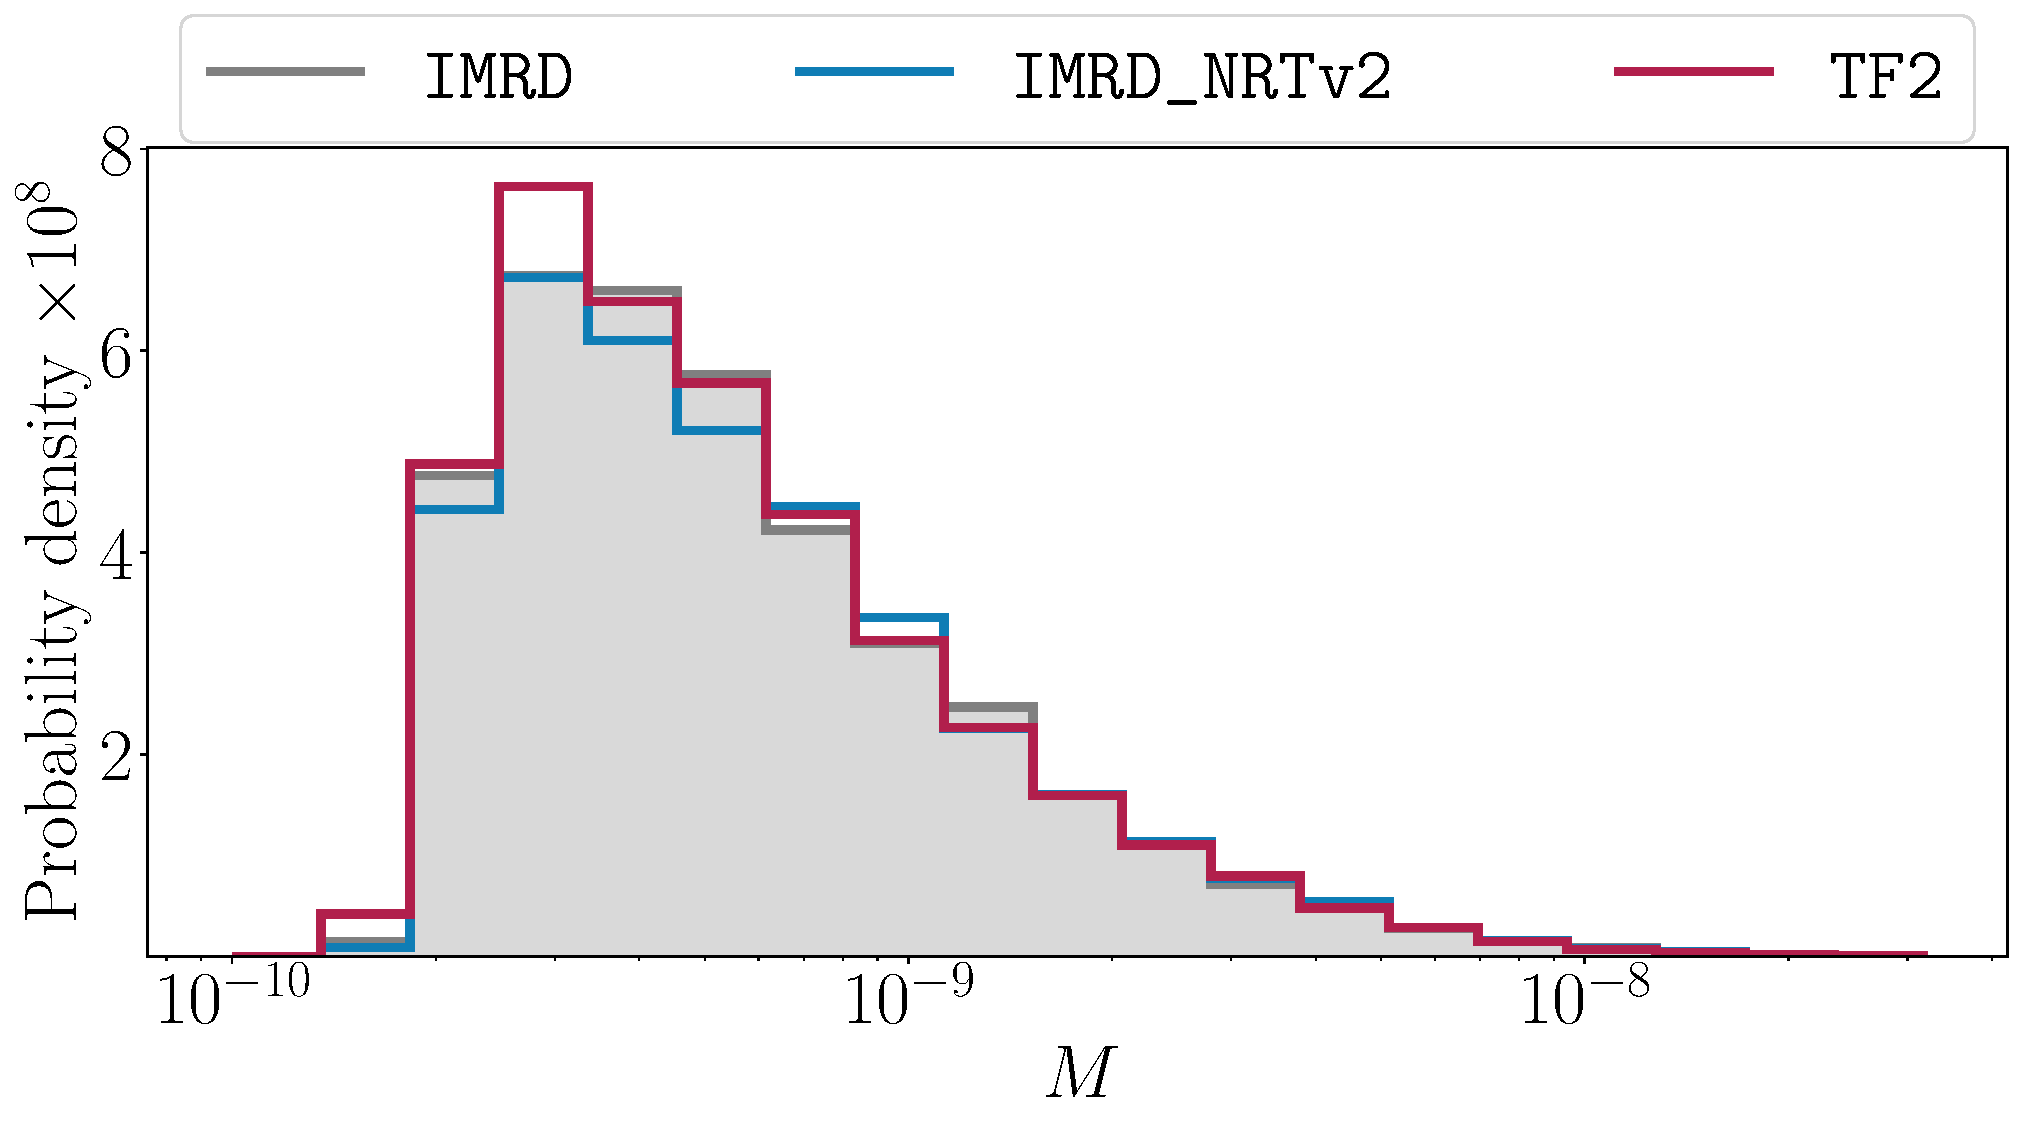
\includegraphics[width=0.7\textwidth]{Figures/mismatch_histogram.pdf}
    \caption*{}
  \end{figure}
  
\end{frame}

\begin{frame}{Priors}
  
  \begin{table}
    \caption{Prior ranges used in our analyses. All priors are uniform priors with the specified range.}
    \label{tab:parameter_priors}
    \renewcommand{\arraystretch}{1}
    % \begin{tabular}{\textwidth}{@{\extracolsep{\fill}} l l l l l}
      \begin{tabular}{l l l l l}
    \hline \hline
    Parameter  & Injection & GW170817 & GW190425 \\ \hline
    $\mathcal{M}$ $[M_\odot]$ & $[0.88, 2.61]$ & $[1.18, 1.21]$ & $[1.485, 1.490]$ \\
    $q$ & $[0.5, 1]$ & $[0.125, 1]$ & $[0.125, 1]$ \\ 
    $\chi_i$ & $[-0.05, 0.05]$ & $[-0.05, 0.05]$ & $[-0.05, 0.05]$ \\
    $\Lambda_i$ & $[0, 5000]$ & $[0, 5000]$ & $[0, 5000]$ \\
    $d_L$ $[\rm{Mpc}]$ & $[30, 300]$ & $[1, 75]$ & $[1, 500]$ \\
    $t_c$ $[\rm{s}]$ & $[-0.1, 0.1]$ & $[-0.1, 0.1]$ & $[-0.1, 0.1]$ \\
    $\phi_c$ & $[0, 2\pi]$ & $[0, 2\pi]$ & $[0, 2\pi]$ \\
    $\cos \iota$ & $[-1, 1]$ & $[-1, 1]$ & $[-1, 1]$ \\
    $\psi$ & $[0, \pi]$ & $[0, \pi]$ & $[0, \pi]$ \\
    $\alpha$ & $[0, 2\pi]$ & $[0, 2\pi]$ & $[0, 2\pi]$ \\
    $\sin \delta$ & $[-1, 1]$ & $[-1, 1]$ & $[-1, 1]$ \\
    \hline \hline
    \end{tabular}
\end{table}
\end{frame}

\begin{frame}{GW170817 \& GW190425: Jensen-Shannon divergences}

  \def\x{-1mm}
  
  \vspace{\x}

  \footnotesize

  \begin{table}
    \centering
    \def\arraystretch{1}
    \caption{Jensen-Shannon divergences (in bits) between the marginal posterior obtained for GW170817 and GW190425 using \texttt{TaylorF2} and \texttt{IMRPhenomD\_NRTidalv2} with \textsc{Jim} and \textsc{pBilby}, with the highest value of each comparison in bold. The divergences are bound between $[0, 1]$.}
    \begin{tabular*}{\textwidth}{@{\extracolsep{\fill}} l  c  c  c  c }

      \hline\hline
& \multicolumn{2}{ c }{GW170817} & \multicolumn{2}{ c }{GW190425} \\
Parameter & \texttt{TF2} & \texttt{NRTv2} & \texttt{TF2} & \texttt{NRTv2} \\ \hline
      
$\mathcal{M}$ & $0.001725$ & $0.000516$ & $0.003557$ & $0.002461$ \\
$q$ & $0.005212$ & $0.007894$ & $0.004837$ & $0.002960$ \\
$\chi_1$ & $0.005633$ & $0.004301$ & $0.002794$ & $0.004825$ \\
$\chi_2$ & $0.003030$ & $0.002671$ & $0.002416$ & $0.003041$ \\
$\Lambda_1$ & $0.001062$ & $0.002208$ & $0.008556$ & $0.000783$ \\
$\Lambda_2$ & $0.000559$ & $0.002186$ & $0.005808$ & $0.003576$ \\
$d_L$ & $0.001544$ & $\bm{0.01847}$ & $0.001273$ & $0.002878$ \\
$\phi_c$ & $0.003500$ & $0.010714$ & $0.003338$ & $0.006126$ \\
$\cos \iota$ & $0.001615$ & $0.012851$ & $0.006400$ & $0.005279$ \\
$\psi$ & $0.004048$ & $0.011036$ & $0.001516$ & $0.003730$ \\
$\alpha$ & $\bm{0.014008}$ & $0.001258$ & $\bm{0.009822}$ & $\bm{0.012291}$ \\
$\sin \delta$ & $0.009570$ & $0.001761$ & $0.008934$ & $0.009228$ \\
\hline\hline
    \end{tabular*}
    \label{tab: JS divergences events}
\end{table}
\normalsize
\end{frame}

\begin{frame}{GW170817 with \texttt{TaylorF2}}
  \vspace{-4.5mm}
  \begin{figure}

    \begin{minipage}[c]{0.2\textwidth}
    \caption{}\label{fig: GW170817 TaylorF2}
    \end{minipage}\hfill
    \begin{minipage}[c]{0.8\textwidth}
    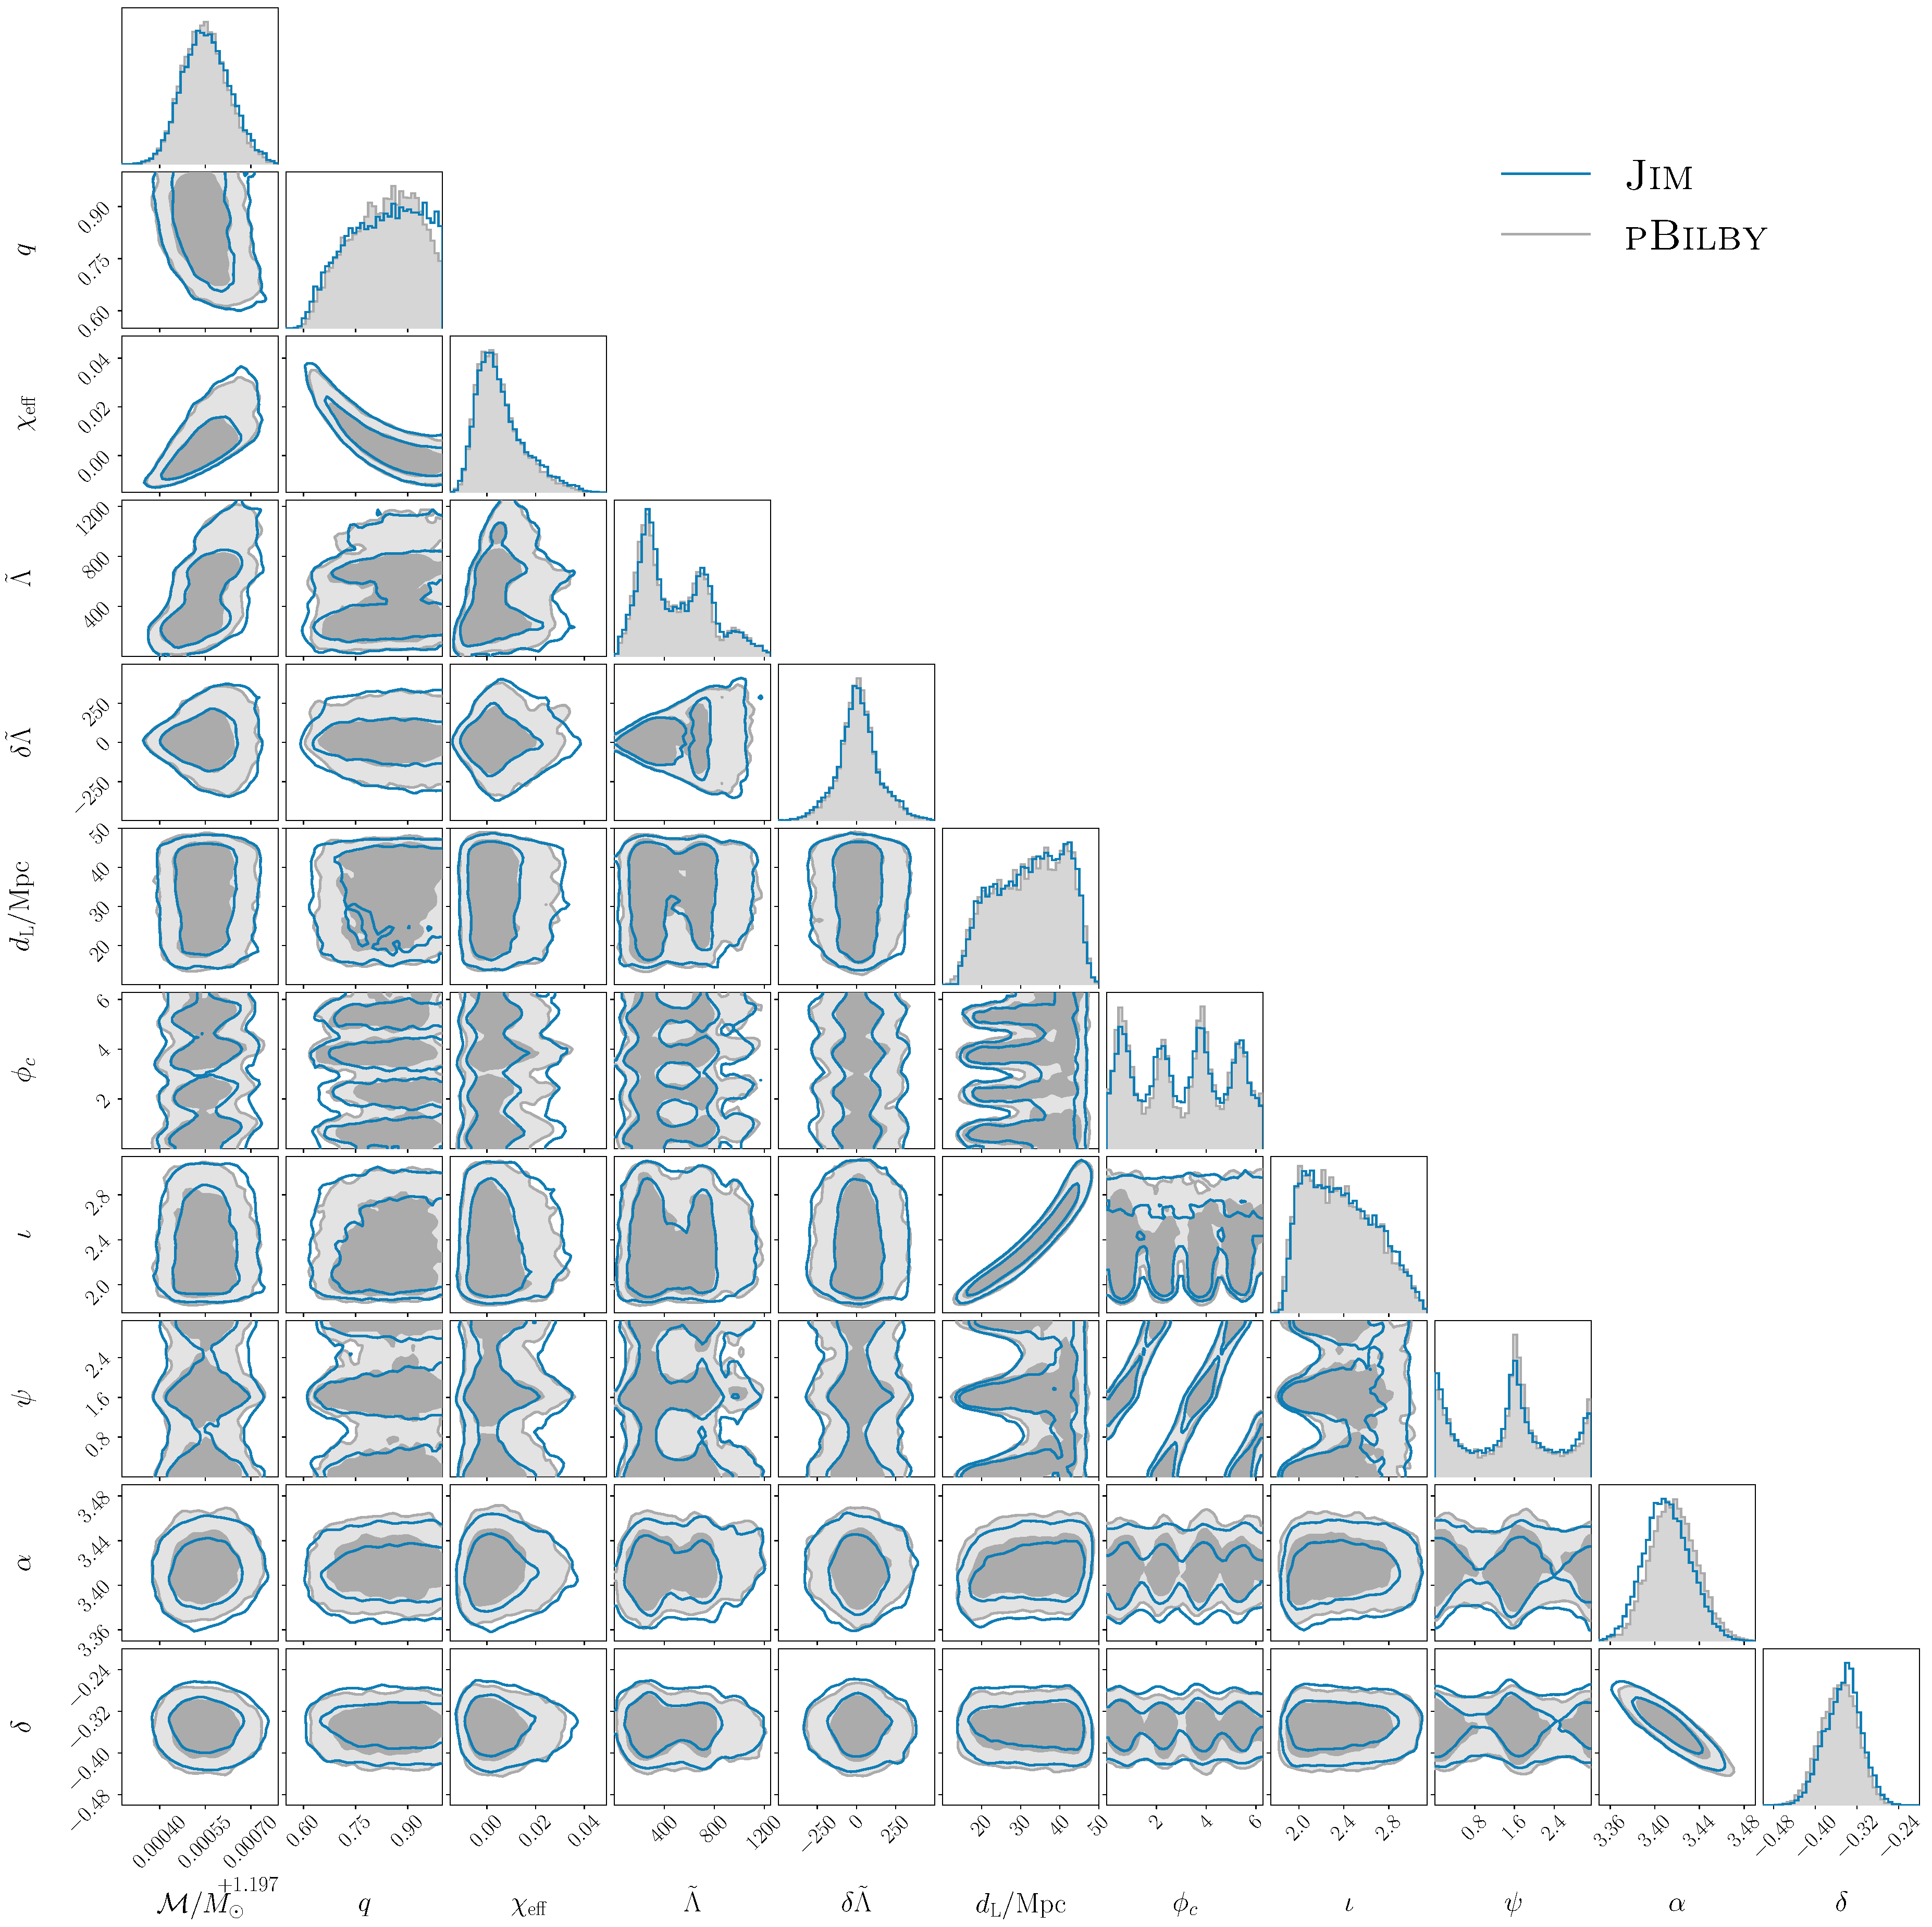
\includegraphics[scale = 0.132]{Figures/GW170817_TaylorF2.pdf}
    \end{minipage}
    
  \end{figure}
\end{frame}

\begin{frame}{GW170817 with \texttt{IMRPhenomD\_NRTidalv2}}
  \vspace{-4.5mm}
  \begin{figure}
  
  \begin{minipage}[c]{0.2\textwidth}
    \caption{}\label{fig: GW170817 NRTidalv2}
    \end{minipage}\hfill
    \begin{minipage}[c]{0.8\textwidth}
    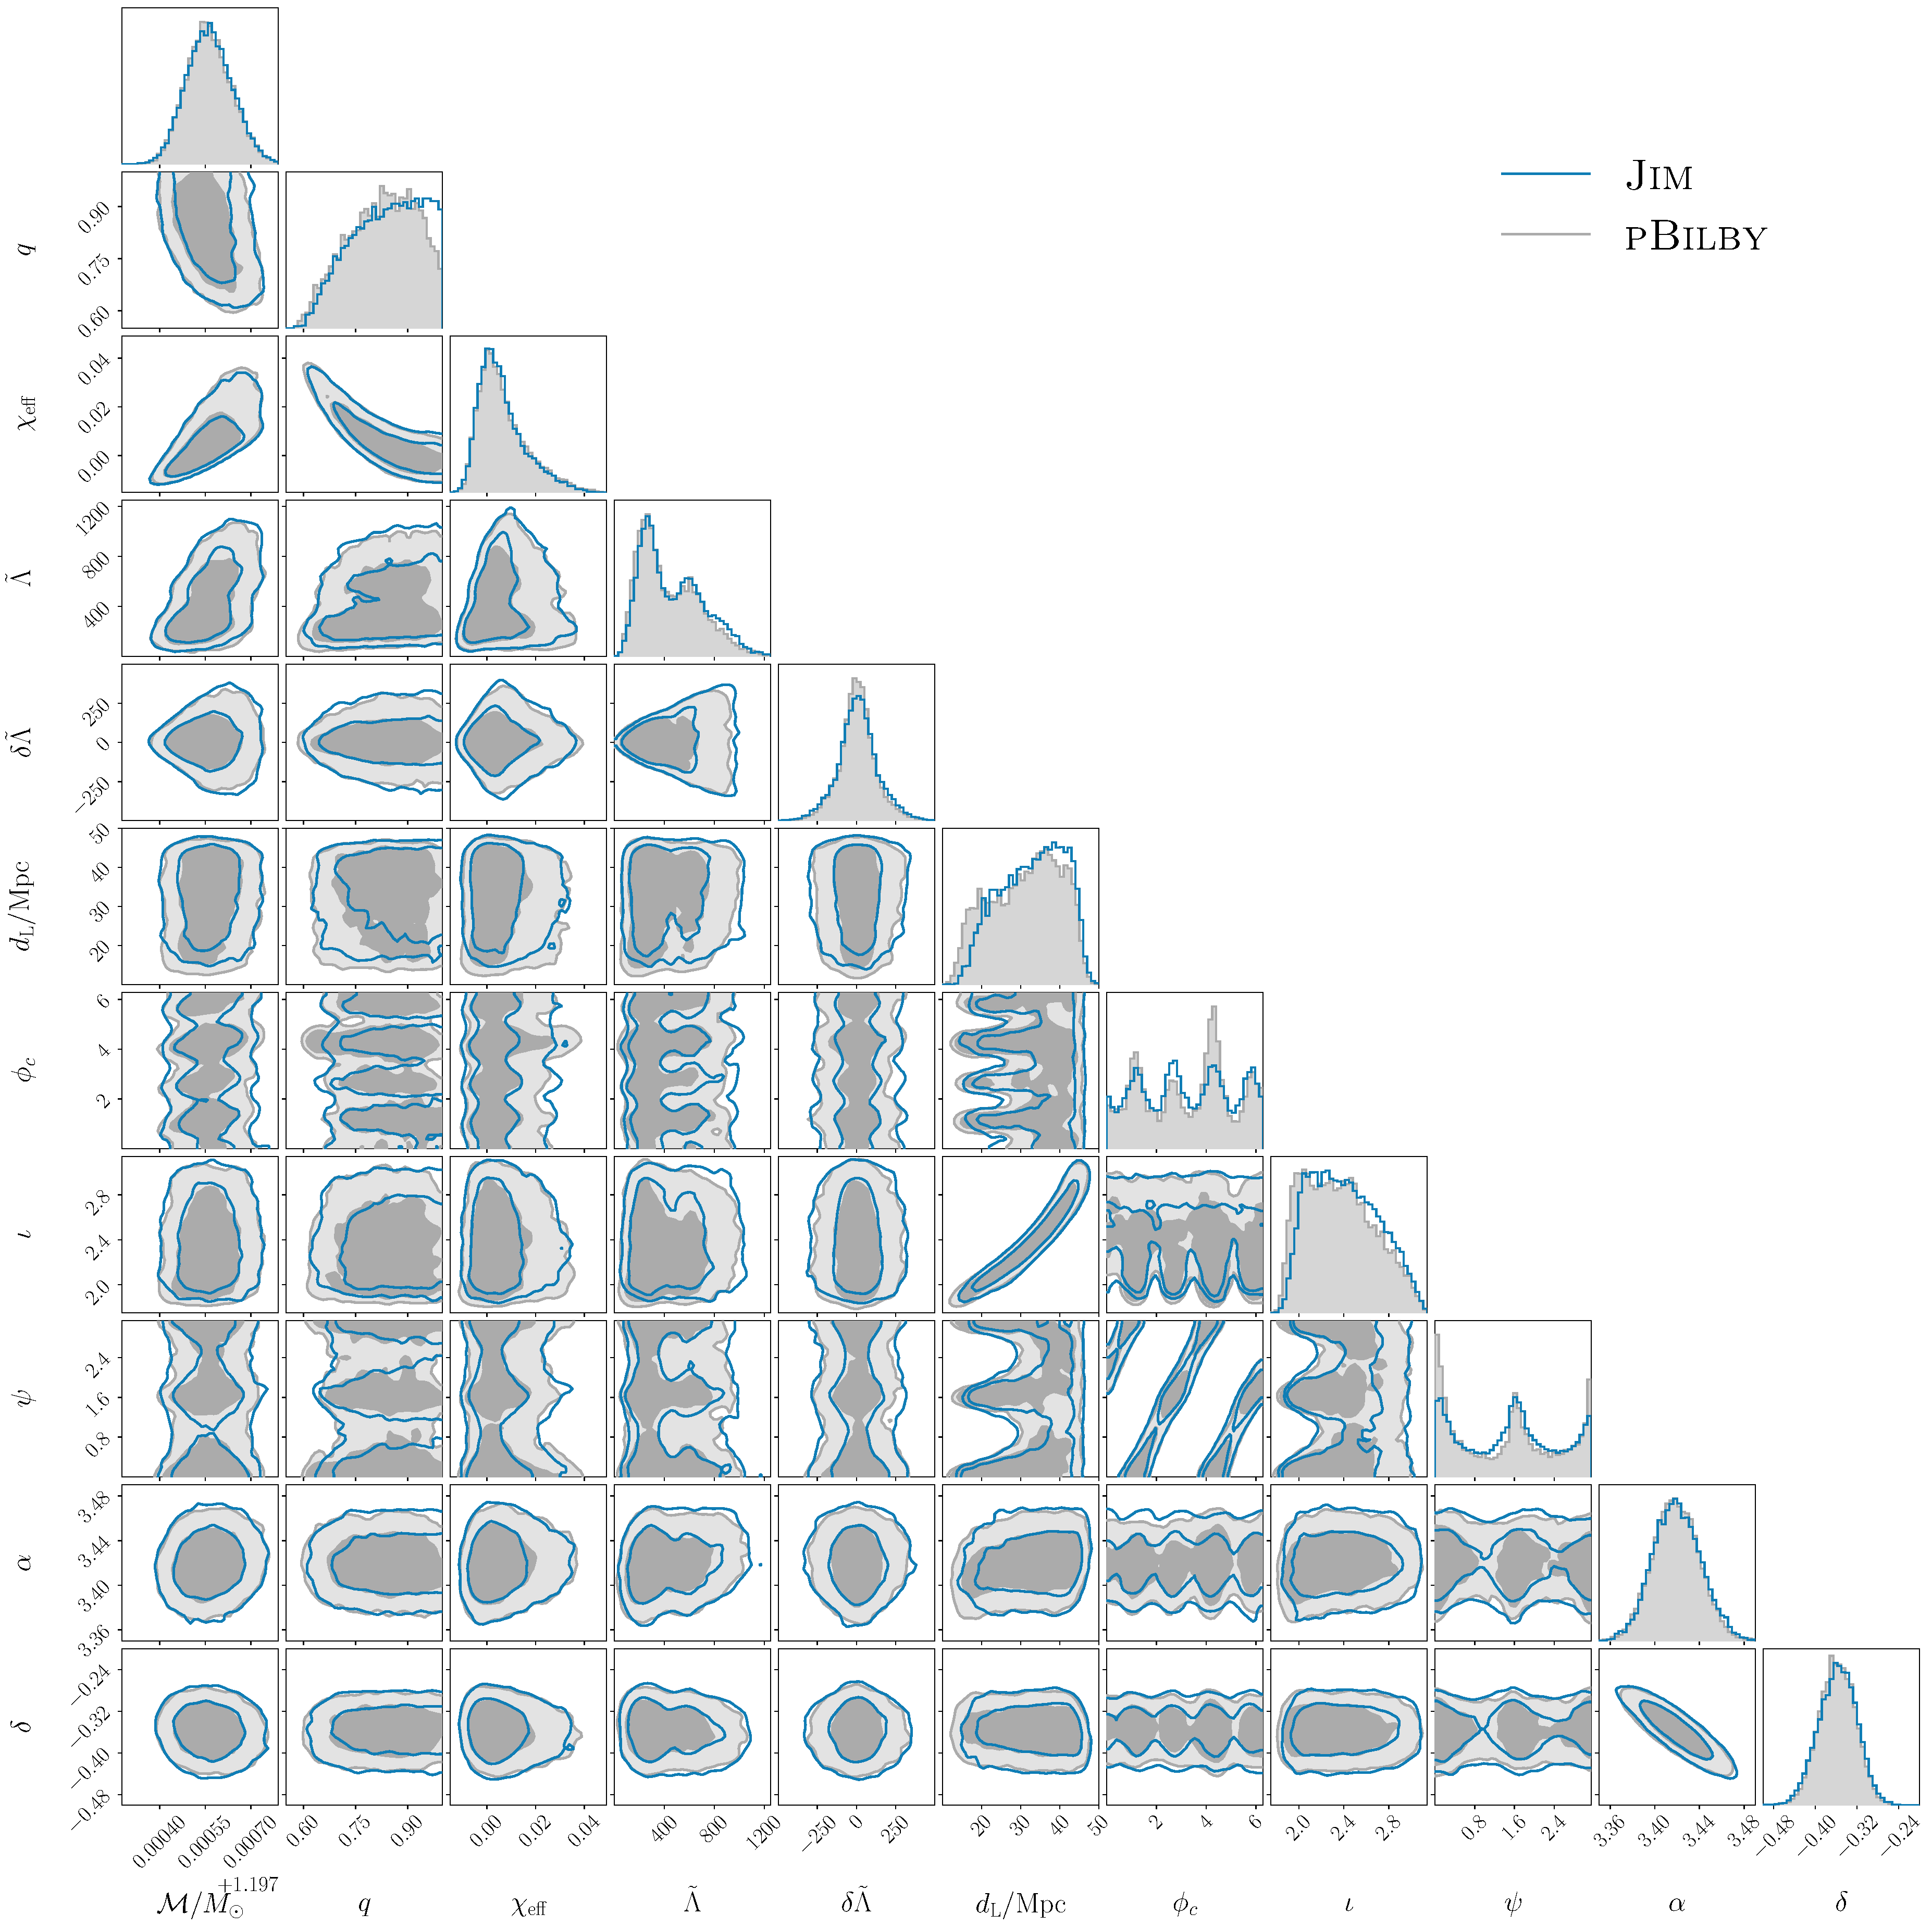
\includegraphics[scale = 0.132]{Figures/GW170817_NRTidalv2.pdf}
    \end{minipage}
  \end{figure}
\end{frame}


\begin{frame}{GW190425 with \texttt{TaylorF2}}
  \vspace{-4.5mm}
  \begin{figure}
  
  \begin{minipage}[c]{0.2\textwidth}
    \caption{}\label{fig: GW190425 TaylorF2}
    \end{minipage}\hfill
    \begin{minipage}[c]{0.8\textwidth}
    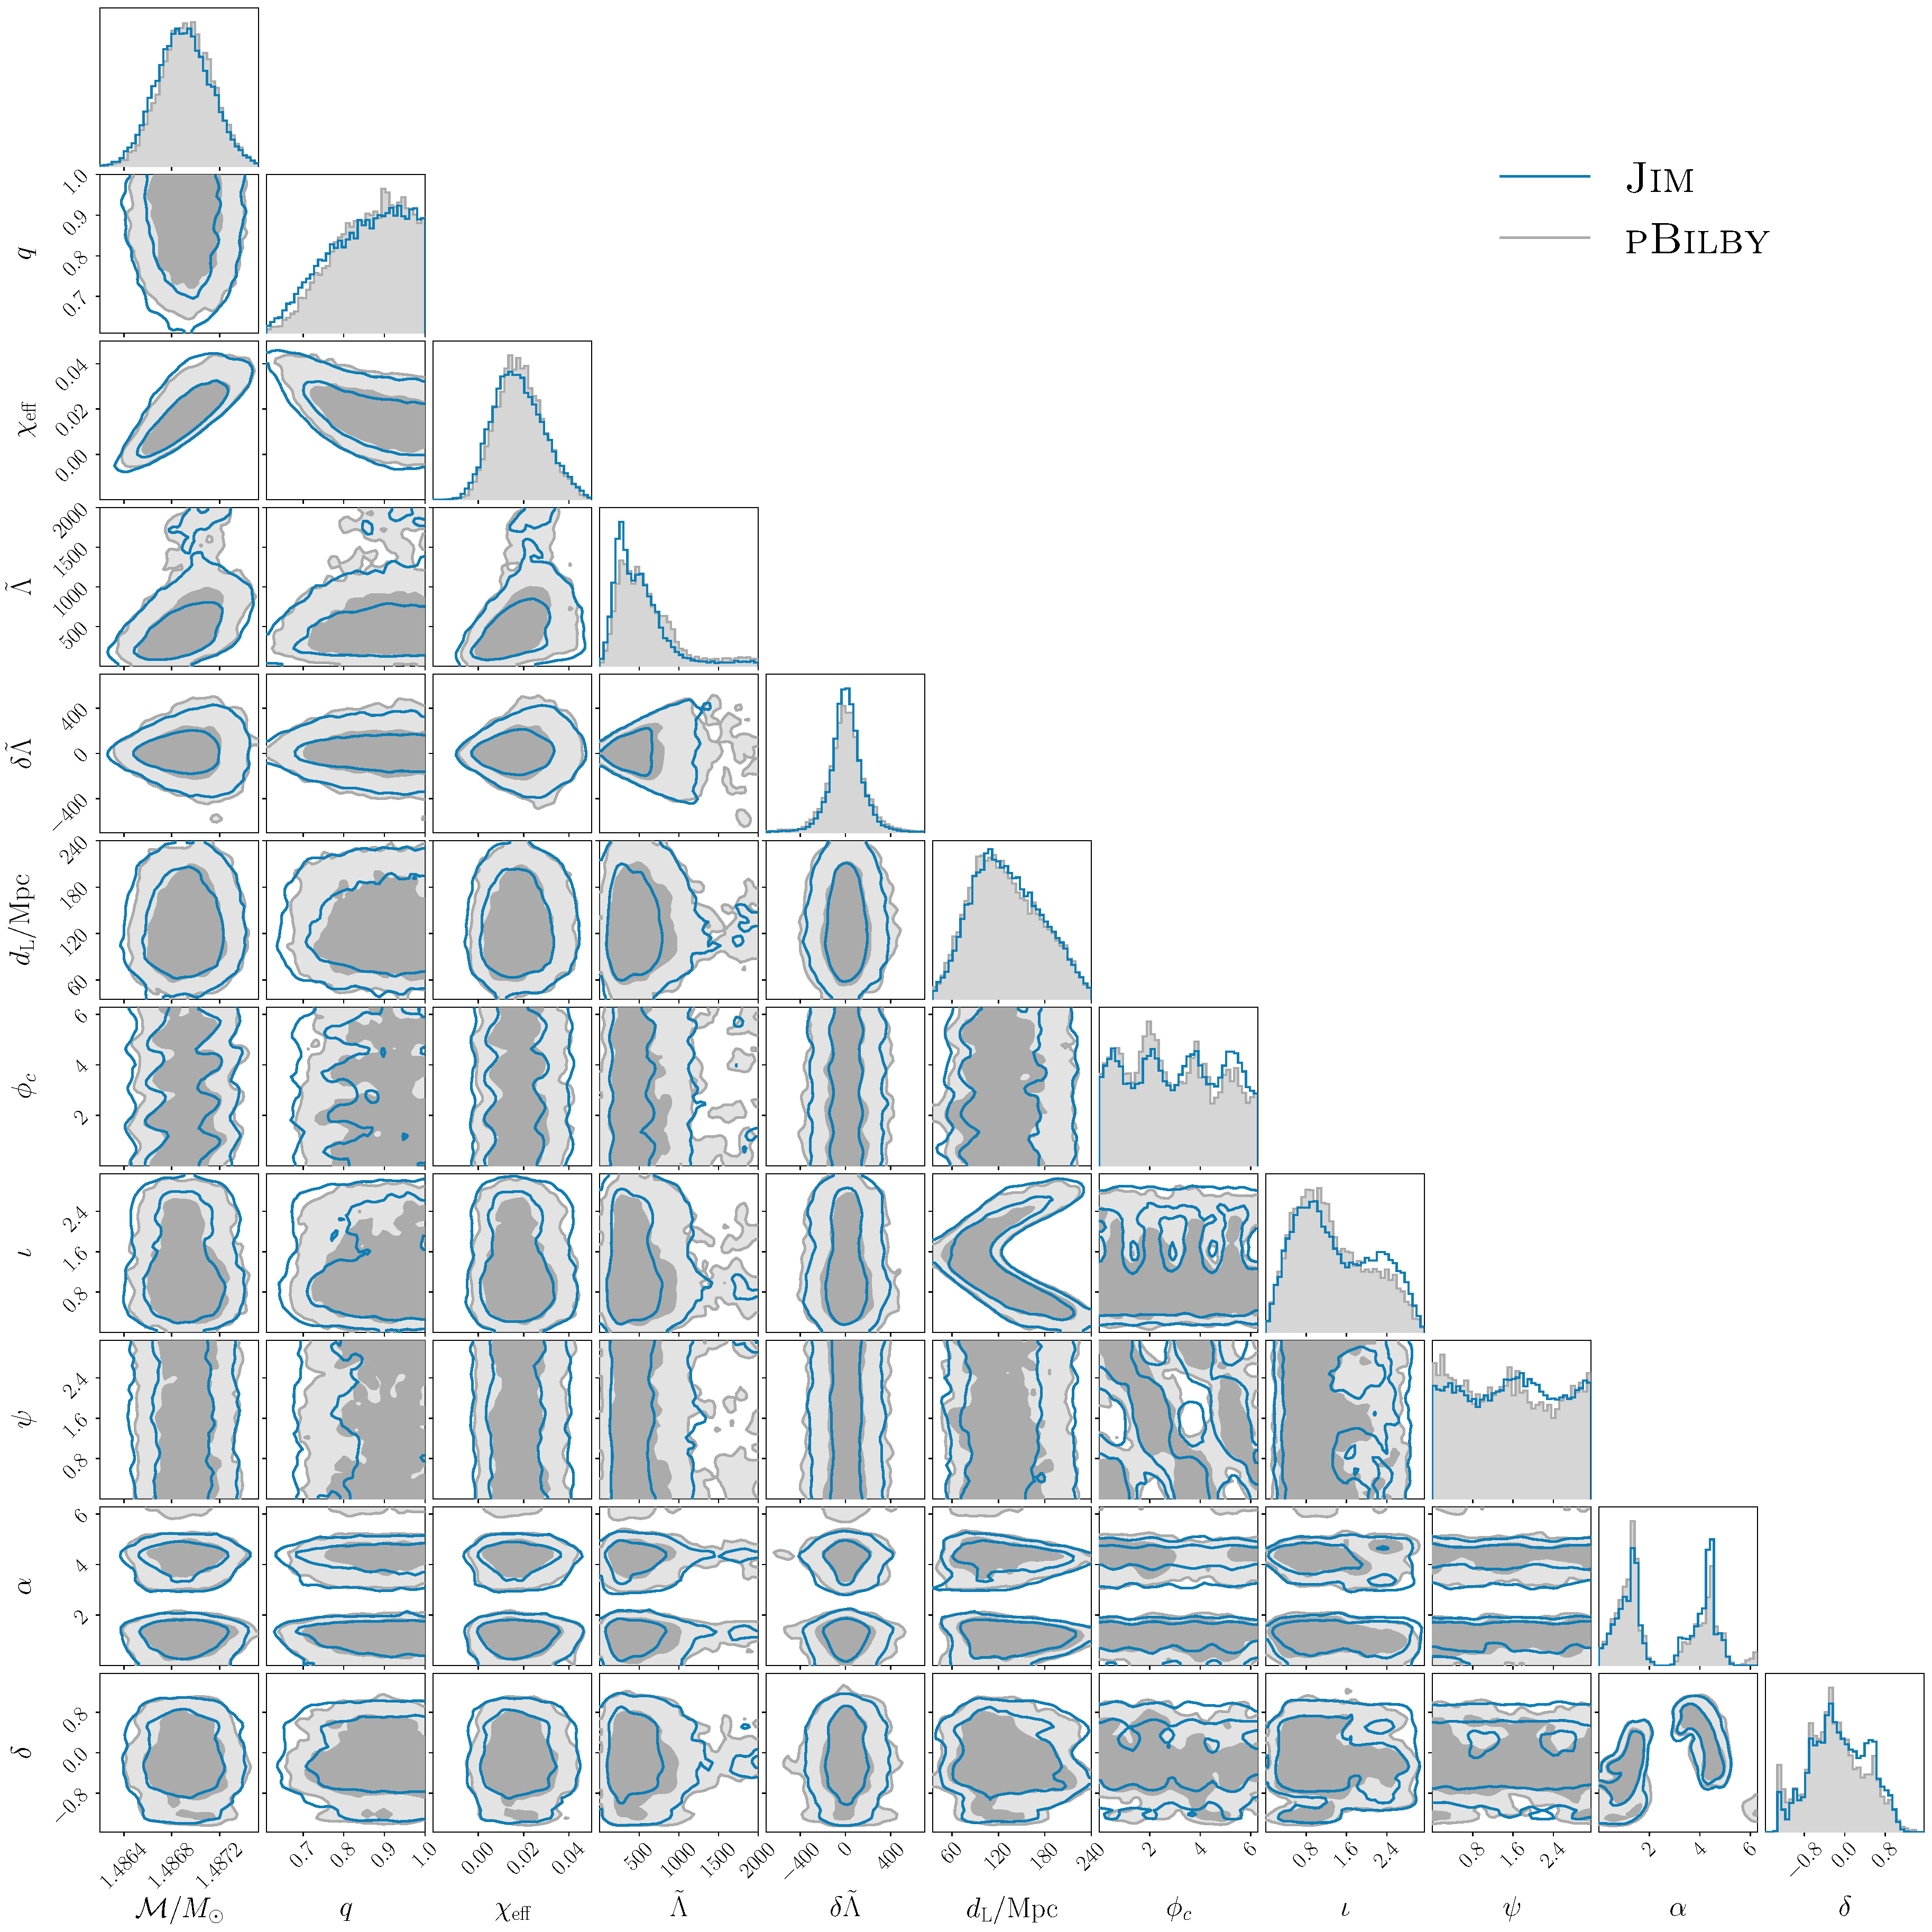
\includegraphics[scale = 0.132]{Figures/GW190425_TaylorF2.pdf}
    \end{minipage}
  \end{figure}
\end{frame}

\begin{frame}{GW190425 with \texttt{IMRPhenomD\_NRTidalv2}}
  \vspace{-4.5mm}
  \begin{figure}
  \begin{minipage}[c]{0.2\textwidth}
    \caption{}\label{fig: GW190425 NRTidalv2}
    \end{minipage}\hfill
    \begin{minipage}[c]{0.8\textwidth}
    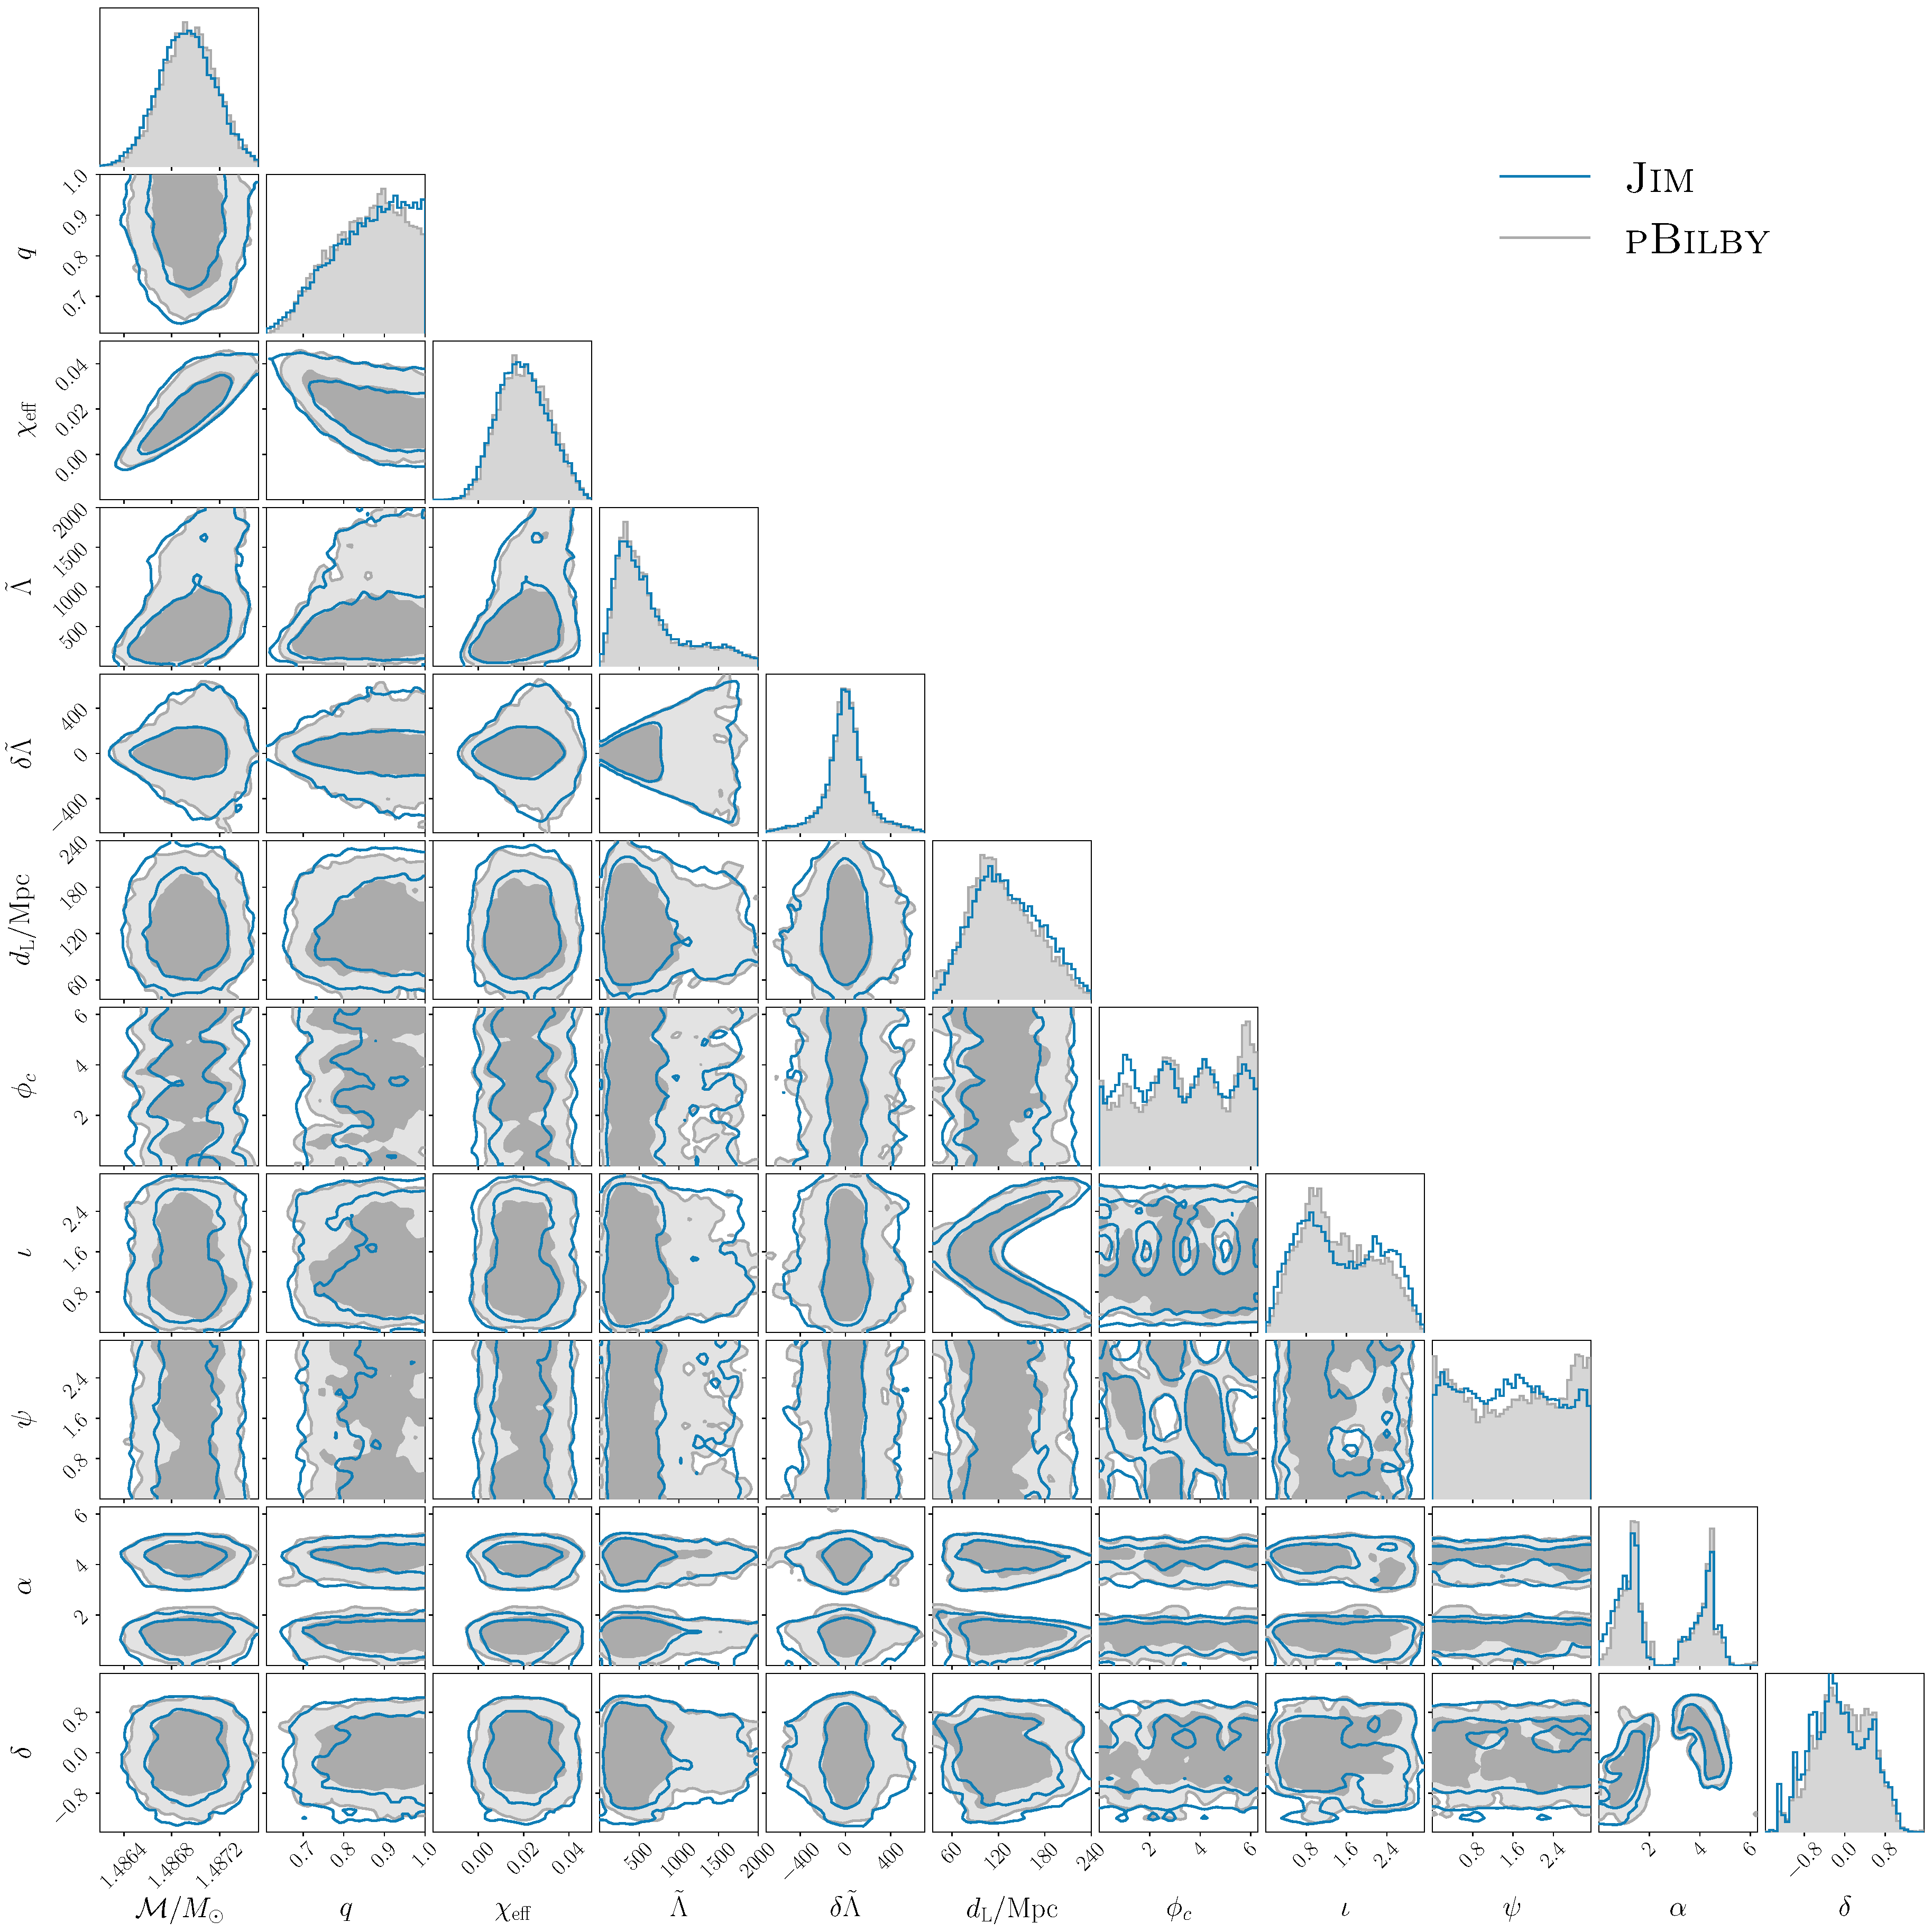
\includegraphics[scale = 0.132]{Figures/GW190425_NRTidalv2.pdf}
  \end{minipage}  
  \end{figure}
  
\end{frame}

\end{document}

